\newpage
\section{Experiments}\label{sec:experiments}

In this section we provide all the details regarding the experimental evaluation done in order to show the performance of the \DPATM\ system. 
We intend to show the suitability of the dynamic pipeline computational model as a real-time system capable of emitting results as they are computed, in a progressive way.\\

First, in \ref{exps:design-of-experiments} we describe the design of the experiments 
that we proposed to study the performance of the \DPATM\ system in different scenarios. 
Then, in Subsection \ref{exps:exps-settings} we describe the running environment.\\

As we already mentioned \ref{sec:prelim}, the system performance is evaluated using several standard metrics namely: 
(i) the response time (\RT) and the average time (\MRT) that measure the exact and average time that the system takes to output a check result, 
from the moment in which the transaction enters the system until the check result is given; 
(ii) the execution time (\ET) that states how fast is the system to process the whole input data stream; 
(iii) the \dieft, that indicates the continuous behavior of the system throughout the execution time and (iv) the throughput (\T) 
(number of results and of interactions emitted by second). 
A detail description of the evaluation metrics is given in \ref{exps:evaluation-metrics}.\\

As mentioned before, due to the sensitive nature of the bank data, to carry our experiments we needed to generate our own synthetic datasets, 
for both the bank database and the stream of transactions. 
In Subsection \ref{exps:datasets} we provide full detail on the generation of our own synthetic bank databases and, 
regarding the transaction stream, we devote the Subsection \ref{exps:bank-stream}, to detail the considered transaction 
streams for our experiments and explain how we performed their generation. 
Finally, in Subsection \ref{exps-input-reading} we discuss different considered methods to consume the stream of transactions, 
and the empirical comparisons from which we decided the method of stream consumption by the \DPATM\ in our experiments. 
Part of this discussion was already advanced in the description of the implementation of the \source\ \Sr\ stage in Section \ref{sec:CQE-DPATM}.\\

In the empirical study we conducted we considered an alternative \emph{result} definition. 
In effect, for our experimental purposes we considered that \emph{results} emitted by the \DPATM\ correspond to \emph{fraud pattern checking}.
That is, all the fraud pattern checking are considered as results on this definition, even if they are negative, i.e. when they do not derive in the creation of an alert. 
Considering all the fraud pattern checking as results is done 
%only due to experimental purposes, 
in order to better analyze the continuous production of results by the \DPATM, 
reflecting all the fraud pattern checking that the system is undergoing. 
Note that, considering all the checking as results induces a communication overhead among  \filter\ \F\ stages and the \sink\ \Sk\ stage, 
where the results are gathered. In a production version of \DPATM\ we would use the original definition of a \DPATM\ system result, i.e. only alerts would be considered results, since sending negative fraud pattern checks to \Sk\ would be of no interest.
%as there would be no interest in sending negative fraud pattern checks to \Sk. 
%Only the positive fraud pattern checks - the alerts - are of interest in that case, 
This means that in a production setting, the overhead in the communication channels among the $\mathsf{F}$'s 
and \Sk\ and the corresponding processing of results in \Sk\ would be reduced at maximum.

\subsection{Design of Experiments}\label{exps:design-of-experiments}

% Explicación breve de los dos principales tipos de experimentos que hemos hecho: RT and NRT-high load scenario
To evaluate the performance of the \DPATM\ we initially proposed two kinds of experiments. On the one hand, the evaluation of the \DPATM\ in scenarios simulating close-to-reality transaction frequencies (E0). On the other hand, the analysis of the \DPATM\ on a high-load stress scenario (E1), where we study the behavior of the system in a worst case scenario, receiving a high loaded transaction stream.\\

\subsubsection{E0: Evaluation in a Real-World Stress Scenario}

This experiment was proposed to evaluate the behavior of the \DPATM\ in a close-to-reality scenario in terms of the frequency of transactions of the input stream that arrive to the system.\\

% 1. Comentar la frequencia de tx
In a real case scenario, the frequency of the transactions on the transaction stream reaching our system will depend mainly on the size of the bank considered. For small-sized banks we do not expect this transaction frequency to be quite high due to its reduced number of clients - and therefore cards - that can perform operations on a certain period of time. On the contrary, for big sized banks we do expect the frequency of transactions to be higher.
In general, we assume that, on average, a cardholder does not perform more than one transaction per day at an ATM. This is indeed the case for the transaction streams that we are going to employ in our experiments, on them the average number of ATM operations per client per day is $\mathsf{0.666}$ (see Table \ref{table:wisabi-average-num-ops} on \ref{exps:datasets}).\\

% 2. Como se pretende simular
To simulate the arrival of transactions with their real frequency, we will feed the system with the transaction stream replicating their actual arrival times. This means maintaining the appropriate time gaps between consecutive transactions. Specifically, for each consecutive pair of interactions ($\mathsf{e_i, e_{i+1}}$), the serving of the second interaction $\mathsf{e_{i+1}}$ to the pipeline will be delayed by the exact time difference from the previous interaction $\mathsf{e_{i}}$.\\

% 4. Problema - baja carga - apenas diferencia entre los sistemas... -> e1
% - O escalabamos o simulabamos un banco mucho mas grande
% 3. Problema - necesidad de escalado, peŕdida de alerts, y realción con el escenario de stress -> e1
For this experiment, we initially considered a small bank database system, \smallG, consisting of 2000 cardholders and 50 ATMs. Considering that each cardholder, on average, does not perform more than one ATM operation per day, we decided to simulate a transaction stream spanning several weeks or months to achieve a reasonable stream size. However, two issues arose: first, performing a single simulation spanning multiple days or months proved impractical due to time constraints; second, we realized that such a low transaction frequency would not yield meaningful insights into the system's performance due to insufficient stress. To address these challenges, we considered two possible solutions:
\begin{itemize}
    \item (i) scaling the transaction stream by mapping it into an equivalent but smaller-sized stream
    \item (ii) considering a larger bank database system
\end{itemize}

We initially applied the \emph{scaling} workaround through some experiments on the \smallG\ database system, with the \smallGThirty\  stream, a transaction stream representing 30 days of simulated activity for the \smallG\ bank. We tested different time scalings, reducing the stream to 12, 6 and 1 hour length. However, we needed to further adapt the scaling by adjusting transaction timestamps to the order of microseconds $\mu s$, as the system was failing to report some expected alerts under the original to the second $s$ scaling. Finally, with this scaling some experiments with the same \smallGThirty\ stream were carried; in particular with a 10 minute length scaling. On Figure \ref{fig:exps-RT-10min-16c} we can see some results of this test. We can observe that the differences between the different \DPATM\ configurations tested with 1, 40 and 2000 filters are almost negligible. On \ref{img:exps-RT-10min-16c-trace-1} the result traces of all the variants are almost identical. And in \ref{img:exps-RT-10min-16c-mrt} the differences in the \MRT\ are also insignificant, in the order of less than 1 or 2 milliseconds. This was due to the still low level of stress to which we were subjecting the \DPATM. \\

\begin{figure}[H]
    \centering
    \hspace{-1.5cm} 
    \begin{subfigure}{0.6\textwidth}
        \centering
        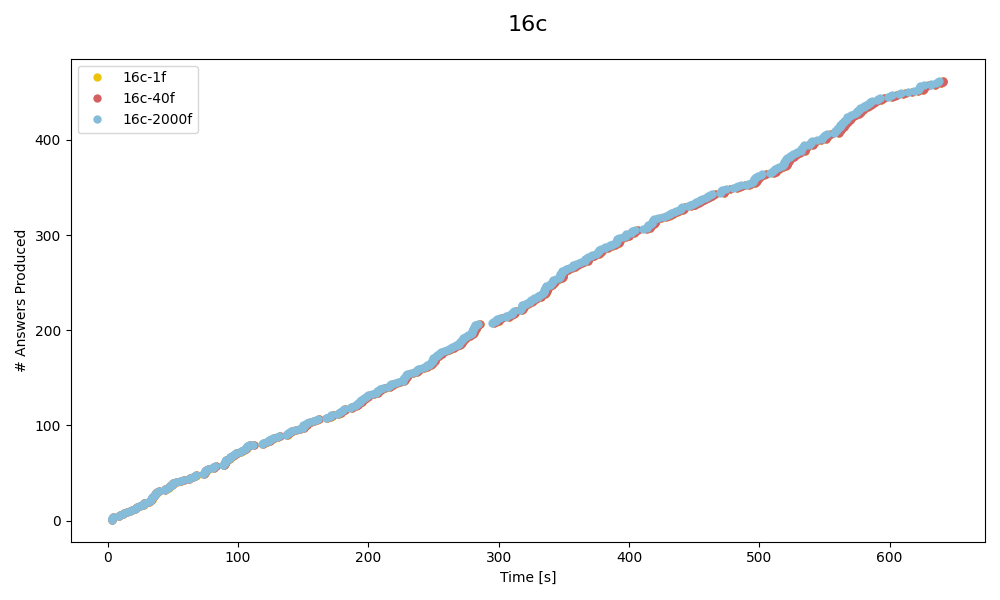
\includegraphics[scale=0.5]{images/4-Experiments/RT-10mins/traces-16c.png}
        \caption{}
        \label{img:exps-RT-10min-16c-trace-1}
    \end{subfigure}
    \hfill
    \begin{subfigure}{0.3\textwidth}
        \centering
        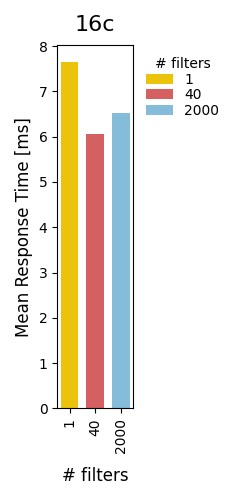
\includegraphics[scale=0.58]{images/4-Experiments/RT-10mins/mrt-16c.png}
        \caption{}
        \label{img:exps-RT-10min-16c-mrt}
    \end{subfigure}
    \hspace{-1cm}
    \caption{For 1, 40 and 2000 number of filters configurations of the \DPATM\ for the \smallGThirty\ input stream test of the \smallG. Run with \texttt{16} cores. (a) Shows the results trace of pairs (result, time(s)). Vertical axis shows the \emph{result} number and horizontal axis shows the time in seconds at which that result is produced. (b) Shows the \MRT\ achieved for the different configurations. On this test, we considered only the alerts as system \emph{results}.}
    \label{fig:exps-RT-10min-16c}
\end{figure}

In summary, we realized that we needed to test the system under a high-load stress scenario (E1), forcing the transaction stream frequency to be as high as possible in order to identify the system's limits.

\subsubsection{E1: Evaluation in a High-Load Stress Scenario}\label{exps-design-e1}

This experiment aims to serve as a means to evaluate the behavior of the \DPATM\ in a high load stress scenario. This scenario is a worst case scenario in terms of the frequency of transactions on the input stream arriving to the system, which will be simulated to be at its maximum peak.\\

% Intención / Objetivo / Qué queremos ver:
In a real case scenario, the frequency of the transactions on the transaction stream reaching our system will depend mainly on the size of the bank considered. For small-sized banks we do not expect this transaction frequency to be quite high due to its reduced number of clients - and therefore cards - that can perform operations on a certain period of time. On the contrary, for big sized banks we do expect the frequency of transactions to be higher. With this, we can claim that this experiment is able to show what would be a real case scenario for a large bank system, where the frequency of transactions occurring in a certain time period is quite high. However, considering that, we can assume that, on average, a cardholder does not perform more than one transaction per day at an ATM 
 - in our considered transactions streams the average number of ATM operations per client per day is $\mathsf{0.666}$ (see Table \ref{table:wisabi-average-num-ops}) - it is important to remark that this scenario would be an unrealistic scenario for most bank systems and that in reality we would expect a lower frequency of transaction input, allowing the \DPATM\ to exhibit a better performance.\\

We will simulate it by providing the \DPATM\ system the transactions of the stream immediately one after the other, as fast as possible. This experiment will be carried considering two bank databases: \smallG, simulating a small bank database system; and \mediumG, simulating a large bank database system. In both cases the stream of transactions is provided at the same speed, the difference lies in the number of cards that each system contains. This will make the \DPATM\ for the large bank system be a \emph{larger} \DPATM, by having to track the activity of more cards. We also expect the time needed to query the stable bank database to be higher in the large bank system.\\

% Cómo lo evaluaré
% Response time - quality of service, que se mantiene
% throughput
% cómo de rápido digiere, interactions/s
% continuous behavior
To evaluate the behavior of the system in this scenario, it is essential to identify the metrics that can tell us how good the system behaves on it. As a real-time system, a key functionality is to be able to emit a response as fast as possible. In our case, to minimize the time to alert the bank system or a user of a potential fraud being produced, being able to minimize the derived damages. A really important metric to measure this is the Response Time, \texttt{RT}, and its average value, the Mean Response Time, \texttt{MRT}.
Also relevant is the evolution of the \texttt{RT} through time, and the evaluation of the continuous behavior of the system through the tested time, measured with the \texttt{dief@t} and \texttt{dief@k} \emph{diefficiency} metrics. Finally, other classical metrics are considered to evaluate the speed at which the system can process a full slice of a stream of transactions: 
the throughput, \texttt{T}, in terms of answers emitted per unit of time and the execution time, \texttt{ET}, to process the full stream. \\

We considered different \DPATM\ configurations regarding the number of filters with which we construct the \DP\ pipeline, 
and we compare the different \DP\ versions against a sequential baseline program. 
These systems were tested for different resources variations, in terms of the dedicated number of cores on which we run them. The description of the results of the experiments performed is detailed on \ref{sec:results}. 

\subsection{Experimental Settings}\label{exps:exps-settings}

\subsubsection{Hardware}

The experiments were run in the machine nodes of the RDLab-UPC cluster at \url{https://rdlab.cs.upc.edu/} \cite{rdlab-upc}. These nodes have different processors: Intel(R) Xeon(R) CPU X5675 @ 3.07GHz and 12
cores, Intel(R) Xeon(R) CPU X5670 @ 2.93GHz and 12 cores, Intel(R) Xeon(R) CPU
X5660 @ 2.80GHz and 12 cores, Intel(R) Xeon(R) CPU X5550 @ 2.67GHz and 8 cores,
and Intel(R) Xeon(R) CPU E5-2450 @ 2.50GHz and 16 cores. We restricted to 16GB of RAM the maximum memory requested to run each 
of the experiments and variate the number of requested cores depending on the experiment. The timeout of each experiment was 24h.\\

% VM Neo4j GDB
Regarding the graph database we used a Neo4j \texttt{5.22.0} (community edition) installed on a virtual machine with 4 cores and 20GB of RAM, 
accessible for the cluster nodes through a \emph{Bolt} protocol on \url{neo4j://10.4.30.227:7687}. 

\subsubsection{Software}

We used the version \texttt{1.20} of the \texttt{Go} language to implement the \DPATM\ system. 
The connection to the Neo4j graph database instance was done using the version \texttt{v5.24.0} of the \texttt{Neo4j Go driver} \cite{neo4j-go-driver-v5240}.\\

Full detail regarding the software used for the implementation of the \DPATM\ system is given in the 
\DPATM-Implementation subsection of Section \ref{ContinuousQueryEngine-Implementation}.

%%

\subsection{Datasets}\label{exps:datasets}

Given the confidential and private nature of bank data, it was not possible to find any real bank dataset. 
In this regard, we had to design and generate our own datasets, comprising the synthetic 
stable property graph bank database and the streams of synthetic transactions.\\

For this, we utilized the synthetic \emph{Wisabi Bank Dataset} \cite{wisabi-bank-dataset} as a base for the construction of our own datasets. 
This dataset could have been adapted to our data model definition and being used it for our experiments. 
However, in order to have full flexibility, and not being constrained to this unique dataset, 
we decided to develop a tool to be able to generate customizable datasets adapted to any experimental needs.\\

\paragraph*{Wisabi Bank Dataset.} The \emph{Wisabi Bank Dataset} is a fictional banking dataset publicly available in the Kaggle platform. 
We used it as a first base to do general customizable programs for the generation of synthetic bank datasets and streams of transactions.\\

The interest to use this bank dataset as a base was mainly because it is large enough dataset and contains card-ATM transactions. 
Additionally, it provides good heterogeneity on the different kind of transactions: withdrawals, deposits, balance inquiries and transfers. Regarding this operations, we gathered the average number of the different kinds of operations performed per cardholder on a day in table \ref{table:wisabi-average-num-ops}. More details of the \emph{Wisabi Bank Dataset} are summarized next.
 
\begin{itemize}
    \item \texttt{8819} customers.
    \item \texttt{50} different ATM locations.
    \item \texttt{2143838} card-ATM transactions records of the different customers during a full year (2022) on five different states of Nigeria (Federal Capital Territory, Lagos, Kano, Enugu and Rivers State).
\end{itemize}

\begin{table}[H]
\centering
\begin{tabular}{|l|l|}
\hline
\multicolumn{1}{|c|}{\textbf{Operation}} & \multicolumn{1}{c|}{\textbf{Value}} \\ \hline
Total operations per day & 0.6660 \\ \hline
Withdrawals per day & 0.3696 \\ \hline
Deposits per day & 0.0742 \\ \hline
Inquiries per day & 0.0743 \\ \hline
Transfers per day & 0.1478 \\ \hline
\end{tabular}
\caption{Wisabi bank dataset average number of the different kinds of operations performed per cardholder on a day}
\label{table:wisabi-average-num-ops}
\end{table}

The dataset consists on ten \emph{csv} tables each with different information which is summarized on Table~\ref{table:wisabi-summary}.

\begin{table}[H]
\centering
\begin{tabular}{|l|l|}
\hline
\textbf{Table}                                                                                               & \textbf{Description}                                              \\ \hline
$\mathsf{enugu\_transactions}$                                                                                 & Transactions of Enugu state (\texttt{350251} transactions)                     \\ \hline
$\mathsf{fct\_transactions}$                                                                                    & Transactions of Federal Capital Territory state \\ & (\texttt{159652} transactions) \\ \hline
$\mathsf{kano\_transactions}$                                                                                   & Transactions of Kano state (\texttt{458764} transactions)                      \\ \hline
$\mathsf{lagos\_transactions}$                                                                                  & Transactions of Lagos state (\texttt{755073} transactions)                     \\ \hline
$\mathsf{rivers\_transactions}$                                                                                 & Transactions of Rivers state (\texttt{420098} transactions)                    \\ \hline
$\mathsf{customers\_lookup}$                                                                                    & Data of the different cardholders (\texttt{8819} cardholders)                 \\ \hline
$\mathsf{atm\_location\_lookup}$                                                                                & Data of the different ATM locations (50 ATMs)                 \\ \hline
\begin{tabular}[c]{@{}l@{}}$\mathsf{calendar\_lookup}$, $\mathsf{hour\_lookup}$,\\ $\mathsf{transaction\_type\_lookup}$\end{tabular} & Complementary data of the previous tables                \\ \hline
\end{tabular}
\caption{Wisabi bank dataset tables summary}
\label{table:wisabi-summary}
\end{table}

The main usage that we did of this dataset was the obtention of a geographical distribution of the ATM locations and the construction 
of a card/client \emph{behavior} based on the ATM-card transactions records provided.

\subsubsection{Synthetic Bank Database Creation}

To do the creation of our synthetic bank database, first we describe the creation of the \emph{csv} files that conform a bank dataset 
and then we describe how the creation and population of the graph database in Neo4j is done.

\paragraph{Bank Dataset Creation: \texttt{bankDataGenerator.py}\\\\}
\label{bankDataGenerator}
\noindent
To generate a bank dataset we developed the Python program \texttt{bankDataGenerator.py}. 
To use it we only need to enter the bank properties' values, and the number of the bank ATMs (internal and external) 
\texttt{n} and Cards \texttt{m} to be generated. With this program we can generate the \emph{csv} files which define 
the bank dataset needed to construct a bank graph database. A directory named \texttt{csv} will be created with the following files: 

\begin{itemize}
    \item \texttt{bank.csv}: bank entity.
    \item \texttt{atm.csv}: ATM entities.
    \item \texttt{card.csv}: card entities.
    \item \texttt{atm-bank-external.csv}: external ATM-bank relations.
    \item \texttt{atm-bank-internal.csv}: internal ATM-bank relations.
    \item \texttt{card-bank.csv}: card-bank relations.
\end{itemize}
To use it:
% How to use the bankDataGenerator

\begin{enumerate}
    \item Ensure to have a \texttt{wisabi} named directory with the \emph{csv} files of the \emph{Wisabi Bank Dataset} (publicly available on Kaggle \cite{wisabi-bank-dataset}).
    \item Ensure to have the \texttt{behavior.csv} file or run \texttt{\$> python3 behavior.py} to create it. This creates a \emph{csv} file with the gathered customer behavior properties from this dataset.
    \item Run \texttt{\$> python3 bankDataGenerator.py} and introduce:
    \begin{enumerate}
        \item Bank properties' values.
        \item $n = |ATM|$, internal and external.
        \item $m = |Cards|$.
    \end{enumerate}
\end{enumerate}

In what follows we give the details on the generation of the instances of the bank dataset entities, as defined in \ref{section:stable-pg}.

\paragraph{Bank: \texttt{bank.csv}\\\\}
\noindent
Since a unique bank instance is considered, the values of the properties of the bank node are manually assigned, 
leaving them completely customizable (see an example on \ref{csv:bank}).

\begin{center}
\lstset{style=csvStyle}
\begin{lstlisting}[caption={Example of a bank.csv}, label={csv:bank}]
                    name,code,loc_latitude,loc_longitude
                    Niger Bank,NIGER,6.478685,3.368442
\end{lstlisting}
\end{center}

\paragraph{ATM: \texttt{atm.csv}\\\\}

\noindent
We generate $\texttt{n = n\_internal + n\_external}$ ATMs (\texttt{n\_internal} ATMs owned by the bank and \texttt{n\_external} external ATMs not owned by the bank, but still accessible
for the bank customers to perform transactions). See an example in \ref{csv:atm}.

\begin{itemize}
    \item \textbf{ATM identifier}: \emph{ATM\_id}. It is assigned a different code depending on the ATM internal or external relation of the ATM with the bank: 
        \[
        \emph{ATM\_id} =
        \begin{cases} 
        bank\_code \text{-} i & 0 \leq i < \texttt{n\_internal } \text{if internal ATM}  \\
        EXT \text{-} i & 0 \leq i < \texttt{n\_external } \text{if external ATM}
        \end{cases}
        \]
    \item \textbf{Geographical properties}: \emph{city}, \emph{country}, \emph{loc\_latitude}         and \emph{loc\_longitude}. 
        They are assigned following the geographical distribution of the locations of the ATMs in the \emph{Wisabi Bank Dataset}. 
        On this dataset there are 50 ATMs locations distributed along Nigerian cities. 
        Note that for each of these ATMs locations, there can be more than one ATMs.
        However, this is not taken into account and only one ATM per location is assumed for the 
        distribution. This distribution of the ATMs matches the relevance of the location in terms of its population, since the number of ATM locations is larger in the most populated 
        Nigerian cities (30\% of the ATM locations are in the city of Lagos, then the 20\% in Kano, and so on). With this, we assign each of the \texttt{n} ATMs \emph{city} and \emph{country} properties a random location/city from the \emph{Wisabi Bank Dataset}, and we then produce random geolocation coordinates inside the bounding box of the city location to set as the \emph{loc\_latitude} and \emph{loc\_longitude} properties of the ATM. \\
\end{itemize}

\begin{center}
\lstset{style=csvStyle}
\begin{lstlisting}[caption={Example of atm.csv}, label={csv:atm}]
                ATM_id,loc_latitude,loc_longitude,city,country
                NIGER-0,12.124651,8.543515,Kano,Nigeria
                NIGER-1,12.148756,8.481764,Kano,Nigeria
                EXT-0,8.941474,7.526291,Abuja,Nigeria
                EXT-1,4.816251,7.010188,Port Harcourt,Nigeria
\end{lstlisting}
\end{center}

\paragraph{Card: \texttt{card.csv}\\\\}

\noindent
We generate a total of \texttt{m} cards that the bank manages. For each of them the assignment of the different properties is done as explained next. An example of a Card data item can be seen in table \ref{table:csv-card-example}.

\begin{itemize}
\item \textbf{Card and client identifiers}:

\[
\begin{cases} 
number\_id = \text{c-}bank\_code\text{-}i \\
client\_id = i 
\end{cases}
0 \leq i < \texttt{m}
\]

\item \textbf{\emph{expiration} and \emph{CVC} properties}: they are not relevant, could be empty value properties indeed or a same toy value for all the cards. The same values are given for all the cards: $expiration = \text{2050-01-17}$, $CVC = 999$.

\item \textbf{Client's habitual address location (\emph{loc\_latitude}, \emph{loc\_longitude})}: two possible options were designed to define the client habitual residence address. In both 
cases they are random 
coordinates drawn from a bounding box of a location/city. The difference is on how the selection of the location/city is done:

  \begin{enumerate}
      \item \textbf{Wisabi customers selection}: take the city/location of the usual ATM of a random selected \emph{Wisabi} database customer. Note that in the \emph{Wisabi Bank Dataset} customers contain an identifier
      of their usual ATM, more in particular, the dataset is designed in such a way that customers
      only perform operations in the same ATM.
      With this approach, we maintain the geographical distribution of the \emph{Wisabi} customers.
      \item \textbf{Generated ATMs selection}: take the city/location of a random ATM of the \texttt{n} generated ATMs. This method is the one utilized so far.
  \end{enumerate}

\item \textbf{\emph{Behavior} properties}: these are properties of special interest both when performing the 
generation of the synthetic transactions of each of the cards and also for the detection of future possible fraud patterns. The defined \emph{behavior} properties are shown in table \ref{table:behavior-properties}. They refer about metrics related with four different types of operations: withdrawal, deposit, balance inquiry and transaction. These operations will be the ones - that, as in the base dataset - considered that a customer can perform when we generate our synthetic transaction dataset.

\begin{table}[H]
    \centering
    \begin{tabular}{|l|l|}
        \hline
        \textbf{Behavior Property} & \textbf{Description} \\ 
        \hline
        $\mathsf{amount\_avg\_withdrawal}$ & Withdrawal amount mean\\ 
        \hline
        $\mathsf{amount\_std\_withdrawal}$ & Withdrawal amount standard deviation \\ 
        \hline
        $\mathsf{amount\_avg\_deposit}$ & Deposit amount mean \\ 
        \hline
        $\mathsf{amount\_std\_deposit}$ & Deposit amount standard deviation\\ 
        \hline
        $\mathsf{amount\_avg\_transfer}$ & Transfer amount mean \\ 
        \hline
        $\mathsf{amount\_std\_transfer}$ & Transfer amount standard deviation \\ 
        \hline
        $\mathsf{withdrawal\_day}$ & Average number of withdrawal operations per day \\ 
        \hline
        $\mathsf{deposit\_day}$ & Average number of deposit operations per day \\ 
        \hline
        $\mathsf{transfer\_day}$ & Average number of transfer operations per day \\ 
        \hline
        $\mathsf{inquiry\_day}$ & Average number of inquiry operations per day \\ 
        \hline
    \end{tabular}
    \caption{\emph{Behavior} properties}
    \label{table:behavior-properties}
\end{table}


The behavior properties' values are assigned to each of the cards by taking a random behavior \emph{row} from the \texttt{behavior.csv} file. This \texttt{behavior.csv} contains the gathered behavior metrics of each of the customers of the \emph{Wisabi Bank Dataset}. It was generated by using the Python program \texttt{behavior.py}. This program creates the behavior of each of the original customers of the \emph{Wisabi Bank Dataset} by doing a summary of all its transaction records on this base dataset.\\

Another possible way to assign the \emph{behavior} parameters could be the assignation
of the same behavior to all of the card instances. However, this method would provide less variability in
the generation of the synthetic transactions than the aforementioned method. 
Nevertheless, other taylored generation methods to generate different \emph{behavior} for 
each the cards could also be considered to similarly obtain this
variability.

\item \textbf{Card money amount extraction limit property}: \emph{extract\_limit}. We set it up by setting an upper bound based on the \emph{amount\_avg\_withdrawal} behavior metric of the card. Other possible ways could be chosen for assigning a value to this property.
    $$extract\_limit: amount\_avg\_withdrawal * 5$$
\end{itemize}

\begin{table}[h]
    \centering
    \lstset{style=csvStyle}
    
    \begin{lstlisting}
    number_id,client_id,expiration,CVC,loc_latitude,loc_longitude,extract_limit
    c-NIGER-0,0,2050-01-17,999,8.92926,7.398833,121590.9
    \end{lstlisting}

    \begin{lstlisting}
    amount_avg_withdrawal,amount_std_withdrawal,withdrawal_day
    24318.18,28174.96,0.2411
    \end{lstlisting}

    \begin{lstlisting}
    amount_avg_deposit,amount_std_deposit,deposit_day,inquiry_day
    11500.0,5889.33,0.0548,0.0493
    \end{lstlisting}

    \begin{lstlisting}
    amount_avg_transfer,amount_std_transfer,transfer_day
    21448.28,20500.15,0.0795
    \end{lstlisting}

    \caption{Example of a Card instance record on the \texttt{card.csv} file}
    \label{table:csv-card-example}
\end{table}


\paragraph{ATM-Bank \texttt{interbank} relation: \texttt{atm-bank-external.csv}\\\\}

To represent the \texttt{interbank} relations between the bank and the external ATMs. Taking the unique ids of each of the related entities, the bank \emph{code} and the \emph{ATM\_id}. Example on \ref{csv:atm-bank-external}.

\begin{center}
\lstset{style=csvStyle}
\begin{lstlisting}[caption={Example of a atm-bank-external.csv}, label={csv:atm-bank-external}]
                                code,ATM_id
                                NIGER,EXT-0
                                NIGER,EXT-1
\end{lstlisting}
\end{center}

\paragraph{ATM-Bank \texttt{belongs\_to} relation:\texttt{atm-bank-internal.csv}\\\\}

To represent \texttt{belongs\_to} relations between the bank and the internal ATMs. Taking the unique ids of each of the related entities, the bank \emph{code} and the \emph{ATM\_id}. Example on \ref{csv:atm-bank-internal}.

\begin{center}
\lstset{style=csvStyle}
\begin{lstlisting}[caption={Example of a atm-bank-internal.csv}, label={csv:atm-bank-internal}]
                                code,ATM_id
                                NIGER,NIGER-0
                                NIGER,NIGER-1
                                NIGER,NIGER-2
\end{lstlisting}
\end{center}

\paragraph{Card-Bank \texttt{issued\_by} relation: \texttt{card-bank.csv}\\\\}

To represent the \texttt{issued\_by} relations between the bank and the card entities. Taking the unique ids of each of the related entities, the bank \emph{code} and the Card id: \emph{number\_id}. Example on \ref{csv:card-bank}.

\begin{center}
\lstset{style=csvStyle}
\begin{lstlisting}[caption={Example of a card-bank.csv}, label={csv:card-bank}]
                                code,number_id
                                NIGER,c-NIGER-0
                                NIGER,c-NIGER-1
                                NIGER,c-NIGER-2
\end{lstlisting}
\end{center}

\paragraph{Bank Database Population\\\\}

To populate the Neo4j graph database instance with the generated bank dataset, we developed the \texttt{populatemodule} \texttt{Go} module. This module takes the bank dataset in the form of the generated \emph{csv} files and populates the indicated Neo4j graph database instance.\\

Two different population modules are proposed. The first, \texttt{csvimport},  does it by directly importing the \emph{csv} files using the \texttt{Cypher}'s \texttt{LOAD CSV} command \cite{cypher-load-csv}, while the second method, \texttt{cypherimport}, does it by parsing the \emph{csv} data and running the creation of the nodes and relationships using \texttt{Cypher} directives. The first method is more convenient whenever we are able to access the file system of the machine in which the Neo4j graph database instance is hosted. Otherwise, the second method provides us an alternative way not needing to access the file system of the machine hosting the Neo4j instance. The module tree structure is depicted in Figure \ref{fig:populatemodule}. On it, the \texttt{cmd} subdirectory contains the scripts to run each of the populating methods: the first method script on \texttt{csvimport} and the second on the \texttt{cypherimport}, while the \texttt{internal} subdirectory is a library of the files with the specific functions used by these methods.\\

\begin{figure}[H]
\centering
\begin{forest}
  for tree={
      font=\ttfamily,              % Typewriter font for file names
      grow'=0,                      % Tree direction (left-to-right)
      child anchor=west,            % Children alignment
      parent anchor=east,           % Parent alignment
      anchor=west,                  % Tree alignment
      calign=first,                 % Aligns with the first child
      edge path={
          \noexpand\path [draw, thick, \forestoption{edge}] (!u.parent anchor) -- +(-1pt,0) |- (.child anchor)\forestoption{edge label};
      },
      inner sep=4pt,
      l=10pt,                       % Level distance
      s sep=5pt                     % Sibling distance
  }
  [populatemodule
      [cmd
        [csvimport
            [main.go]
            [.env]
        ]
        [cypherimport
            [main.go]
            [.env]
        ]
      ]
      [internal
          [common
              [common.go]
          ]
          [populate
              [populate.go]
          ]
      ]
  ]
\end{forest}
\caption{\texttt{populatemodule} file structure}
\label{fig:populatemodule}
\end{figure}

% How to run it - .env file
% Description of each of the methods

To indicate the Neo4j graph database instance to be populated we need to first set up correctly the \texttt{.env} file (see the listing \ref{population-env}) located inside the desired method subdirectory, where we have to define the corresponding Neo4j environment variables \emph{URI}, \emph{username} and \emph{password} to access the Neo4j graph database instance.

\begin{center}
\lstset{style=cypherStyle}
\begin{lstlisting}[caption={Example of a \texttt{.env} file, from which the connection credentials will be gathered by our \texttt{populatemodule}.}, label={population-env}]
                NEO4J_URI="bolt://localhost:7687"
                NEO4J_USERNAME="neo4j"
                NEO4J_PASSWORD="xxxxx"
\end{lstlisting}
\end{center}

Both methods, before doing the population of the Neo4j instance with the \emph{csv} files, perform the creation of uniqueness constraints on the properties of the nodes that we use as our \emph{de facto} IDs for the ATM and Card IDs: \texttt{ATM\_id} and \texttt{number\_id}, respectively. The reason to do this is to avoid having duplicated nodes of these types with the same ID in the database. Therefore, as an example, when adding a new ATM node that has the same \texttt{ATM\_id} as another ATM already existing in the database, we are aware of this and we do not let this insertion to happen. ID uniqueness constraints are created with the following \texttt{Cypher} directives:

\begin{center}
\lstset{style=cypherStyle}
\begin{lstlisting}[caption={Uniqueness ID constraints}]
            CREATE CONSTRAINT ATM_id IF NOT EXISTS
            FOR (a:ATM) REQUIRE a.ATM_id IS UNIQUE
    
            CREATE CONSTRAINT number_id IF NOT EXISTS
            FOR (c:Card) REQUIRE c.number_id IS UNIQUE
    
            CREATE CONSTRAINT code IF NOT EXISTS
            FOR (b:Bank) REQUIRE b.code IS UNIQUE
\end{lstlisting}
\end{center}

Finally, we include a brief description on how to run each of the described population methods of the module:

\begin{itemize}
\item{\texttt{csvimport}: Cypher's \texttt{LOAD CSV}}\\
We use the \texttt{LOAD CSV} clause which directly allows to load \emph{csv}'s into Neo4j, creating the nodes and relations expressed on the \emph{csv} files of the dataset.
To use this method simply follow these steps:
\begin{enumerate}
    \item Place all the CSVs (\texttt{atm.csv}, \texttt{bank.csv}, \texttt{card.csv}, \texttt{atm-bank-internal.csv}, \texttt{atm-bank-external.csv} 
    and \texttt{card-bank.csv}) under the \texttt{/var/lib/neo4j/import} directory
    of the machine containing the Neo4j graph database instance.
    \item Run \texttt{\$> go run populatemodule/cmd/csvimport/main.go}
\end{enumerate}

\item {\texttt{cypherimport}: \emph{Manual} \texttt{Go} parsing\\}
On this method we parse the data of the \emph{csv} files in our \texttt{Go} program, and then, for each record we run a \texttt{Cypher} command to import it as a node instance or relationship in the Neo4j database. This method allow us to avoid locating the \emph{csv} dataset files on the machine where the Neo4j graph database instance is running (in the case it runs in a different machine)
To use this method do:

\begin{itemize}
    \item Run \texttt{\$> go run populatemodule/cmd/cypherimport/main.go <csvPath>}\\ providing as argument \texttt{<csvPath>} the path of the directory where the \emph{csv} dataset files are located.
\end{itemize}

\end{itemize}

\subsubsection{Synthetic Transaction Stream Generation}\label{datasets:transactionstream}

% Details on the process. How the generation is done.
% How to run.
% Files generated. Show example of the csv.

The transaction set constitutes the simulated input data stream continuously arriving to the system. Each transaction represents the operation done by a client's card on a ATM of the bank network with the form of an \emph{interaction} edge/relation of the volatile subgraph (see \ref{section:volatile-pg}) matching one Card with one ATM of the bank database. In what follows we explain the generation of the transaction stream that we employed in order to test our system. Note that, in any case, this is only a possible proposal done with the intention of reproduce a close-to-reality card-ATM bank transaction stream.\\

We divide the generation of the transaction set in the generation of two subsets: the regular transaction set and the anomalous transaction set. The regular transaction set consists of the \emph{ordinary/correct} transactions, that are guaranteed to not produce any anomalous scenario, whereas the anomalous transaction set is composed of the \emph{irregular/anomalous} transactions that are intentionally created to produce the anomalous scenarios. The main reason to do this separation on the generation is to divide the creation of the full transaction stream in two steps. First the creation of the regular transaction stream set, having the control to ensure that no anomalous fraud scenarios are produced in between the transactions of this set. And second, and only after the creation of the regular transaction set, we create the anomalous transaction set, creating transactions that originate anomalous fraud scenarios over the regular transaction set. The union of both sets will form the final generated transaction stream.

\paragraph{Regular Transaction Set\\\\}

The main idea of the creation of this set, is to produce a set of ordinary transactions for each of the cards that do not produce any anomalous scenarios between them. So far, since we are only considering the fraud pattern I for our proof of concept system, the constraints that we need to impose on the generation of the regular transaction set are:

\begin{enumerate}
    \renewcommand{\labelenumi}{\Roman{enumi}.}  
    \item \textbf{Fraud pattern I}: No two consecutive transactions for a card in different ATM locations can be produced with an insufficient feasible time difference.
\end{enumerate}

As a summary of the regular transaction set generation method that we developed, we provide a pseudocode on the Algorithm \ref{alg:regular-tx-generator}. Some of its parts are later explained in detail.\\

The generation of the transaction stream is performed for a customizable \texttt{NUM\_DAYS} number of days starting in a \texttt{START\_DATE} for each of the cards on our bank network. For each card, we take its gathered behavior (see table \ref{table:behavior-properties}) to determine the number and type of interactions performed in the defined days time interval: $[\texttt{START\_DATE}, \texttt{START\_DATE} + \texttt{NUM\_DAYS}]$. The interactions are generated by linking the card to ATMs that are no farther than \texttt{MAX\_DISTANCE\_SUBSET\_THRESHOLD} kilometers from the residence location, \texttt{residence\_loc}, of the client of the card, represented by the location coordinates of the card entity: $(loc\_latitude, loc\_longitude)$. Nevertheless, in a simpler version of the transaction generator program we also consider avoiding this limitation and allow to link the card to any ATM of the bank dataset.
Finally, the interactions are distributed along the defined time interval $[\texttt{START\_DATE}, \texttt{START\_DATE} + \texttt{NUM\_DAYS}]$ respecting the constraint related with the fraud pattern I.

\begin{algorithm}[H]
  \small
  \begin{algorithmic}[1]
  \STATE $\texttt{id} \gets 0$
  \FOR{\text{card} in \text{cards}}
    \STATE $\texttt{ATM\_subset}, \overline{\texttt{ATM\_subset}} \gets \text{createATMsubset(\texttt{residence\_loc})}$
    \STATE $\texttt{t\_min\_subset} \gets \text{calculate\_t\_min\_subset(\texttt{ATM\_subset})}$
    \STATE $\texttt{num\_tx} \gets \text{decide\_num\_tx()}$
    \STATE $T \gets \text{distribute}(\texttt{num\_tx}, \texttt{t\_min\_subset})$
    \FOR{$t_i$ in $T$}
        \STATE $\texttt{ATM}_{i} \sim \texttt{ATM\_subset}$
        \STATE $\texttt{start}_{i} \gets t_i.start$
        \STATE $\texttt{end}_{i} \gets t_i.end$
        \STATE $\texttt{type}_{i} \gets \text{getType()}$
        \STATE $\texttt{amount}_{i} \gets \text{getAmount(}\texttt{type}_{i}\text{)}$
        \STATE $\texttt{id}_{i} \gets \texttt{id}; \ \texttt{id} \gets \texttt{id} + 1$
        \STATE $\text{createTransaction}(\texttt{id}_{i}, \texttt{ATM}_i, \texttt{start}_{i},\texttt{end}_{i}, \texttt{type}_{i}, \texttt{amount}_i)$
    \ENDFOR
    \STATE $\text{introduceAnomalous}(\texttt{ATM\_subset}, \overline{\texttt{ATM\_subset}})$ \COMMENT{Anomalous transaction set}
  \ENDFOR
  \end{algorithmic}
  \caption{Regular Transactions Generation}
  \label{alg:regular-tx-generator}
\end{algorithm}

In what follows we give full detail of each of the steps of the Algorithm \ref{alg:regular-tx-generator}, to complete the explanation of the regular transaction set generation method.

\begin{enumerate}
    \item \textbf{Selection of ATMs}:
    {\footnotesize \textcolor{teal}{$\texttt{ATM\_subset}, \overline{\texttt{ATM\_subset}} \gets \text{createATMsubset(\texttt{residence\_loc})}$}}

    \texttt{ATM\_subset} is the subset of ATMs of the stable bank dataset. It will consist of the ATMs in which we will allow the interactions of a card to occur. We set a limit on the size of this subset, considering only a maximum ratio of the total number of ATMs of the bank network (\texttt{MAX\_SIZE\_ATM\_SUBSET\_RATIO} $\in [0,1]$), so that only a certain amount of the ATMs are included on it: 
    $$|\texttt{ATM\_subset}| = \texttt{MAX\_SIZE\_ATM\_SUBSET\_RATIO} * |\texttt{ATM}|$$ 

    There are two options for the construction of this subset:
    \begin{itemize}
        \item \textbf{\emph{Neighborhood} location selection}: Only the closest $|\texttt{ATM\_subset}|$ ATMs to the cardholder residence location \texttt{residence\_loc} = \emph{(loc latitude, loc longitude)} are included in the subset. These ATMs are considered to be \textit{usual} / belonging to the neighborhood of the cardholder, in terms of its location distance. Apart from the subset size limitation, a maximum distance constraint defined by the
        \texttt{MAX\_DISTANCE\_SUBSET\_THRESHOLD} parameter is imposed:
        
        \begin{align*}
        \texttt{ATM\_subset} &= \{\texttt{ATM}\ |\ \texttt{distance(ATM, residence\_loc)} \\
        &\leq \texttt{MAX\_DISTANCE\_SUBSET\_THRESHOLD}\}
        \end{align*}
    
        \item \textbf{Random selection}: The \texttt{ATM\_subset} is built by randomly selecting $|\texttt{ATM\_subset}|$ ATMs from the considered bank network.
    \end{itemize}

    \item \textbf{Calculate minimum time distance (\texttt{t\_min\_subset})}:\\
    {\footnotesize\textcolor{teal}{$\texttt{t\_min\_subset} \gets \text{calculate\_t\_min\_subset(\texttt{ATM\_subset})}$}}

    \texttt{t\_min\_subset} is the minimum time difference needed to respect between any two consecutive transactions of a card in the regular transaction set. That is, \texttt{t\_min\_subset} is the minimum time distance between the end of a transaction and the start of the next consecutive transaction of a card, needed to guarantee in order to ensure that the constraint I is respected on the generation of the regular transactions set.
    
    $$\texttt{t\_min\_subset} = \frac{\texttt{max\_distance\_subset}}{\texttt{REGULAR\_SPEED}}$$

    To calculate it, we take the time needed to traverse the maximum distance between any pair of ATMs of the \texttt{ATM\_subset}: \texttt{max\_distance\_subset} km at an assumed speed that any two locations can be traveled in the case of regular transaction scenarios: \texttt{REGULAR\_SPEED} km/h.

    \item \textbf{Select the number of transactions \texttt{num\_tx}}:
    {\footnotesize \textcolor{teal}{$\texttt{num\_tx} \gets \text{decide\_num\_tx()}$}}
    
    Based on the behavior of the card, we decide the number of transactions \texttt{num\_tx} to generate for the card for the defined days time interval $[\texttt{START\_DATE}, \texttt{START\_DATE} + \texttt{NUM\_DAYS}]$ using a Poisson distribution as:

    $$\texttt{num\_tx} \sim \text{Poisson}(\lambda = \texttt{ops\_day} * \texttt{NUM\_DAYS})$$ where \texttt{ops\_day} is the sum of the average number of all the kinds of operations per day of the card - client - behavior: 
    $$\texttt{ops\_day} = \texttt{withdrawal\_day} + \texttt{ deposit\_day} + \texttt{ inquiry\_day} + \texttt{ transfer\_day}$$

    \item \textbf{Time distribution of the \texttt{num\_tx} transactions}: 
     {\footnotesize \textcolor{teal}{$T \gets \text{distribute}(\texttt{num\_tx}, \texttt{t\_min\_subset})$}}
    
    Along the selected time interval $[\texttt{START\_DATE}, \texttt{START\_DATE} + \texttt{NUM\_DAYS}]$ we do a random uniform distribution of the \texttt{num\_tx} transactions. $T$ contains the list of all the \texttt{start} and \texttt{end} times tuples for each of the \texttt{num\_tx} transactions, respecting the constraint I: ensuring that, for the considered card, no two consecutive transactions $tx_i$ and $tx_{i+1}$ performed in any of the ATMs of the \texttt{ATM\_subset} are at a time distance lower than \texttt{t\_min\_subset}. Specifically, the transaction times are generated guaranteeing:

    $$tx_i.\texttt{end} + \texttt{t\_min\_subset} < tx_{i+1}.\texttt{start} \ \forall i \in [1,\texttt{num\_tx})$$

    The \texttt{end} time of a transaction is assigned a shifted time difference with respect to the \texttt{start} time. In particular:

    $$
    \texttt{end} = \texttt{start} + \texttt{time\_difference}
    $$

    where:

    $$\texttt{time\_difference} \sim \mathcal{N}(\texttt{MEAN\_DURATION},\,\texttt{STD\_DURATION})$$ with the corrections:

    $$
    \texttt{time\_difference} =
    \begin{cases} 
        \texttt{MEAN\_DURATION} & \text{if } \texttt{time\_difference} < 0 \\
        \texttt{MAX\_DURATION} & \text{if } \texttt{time\_difference} > \texttt{MAX\_DURATION} \\
        \texttt{time\_difference} & \text{otherwise}
    \end{cases}
    $$
    \item \textbf{Assignment of the remaining properties' values:\\}
    Once all the previous steps are done, the remaining values for the properties of each of the \texttt{num\_tx} transactions are assigned (this corresponds to the lines 7-15 in the algorithm pseudocode \ref{alg:regular-tx-generator}). For each of the transactions:
    \begin{itemize}
        \item \textbf{Link to a random ATM of the \texttt{ATM\_subset}}\\
        {\footnotesize \textcolor{teal}{$\texttt{ATM}_{i} \sim \texttt{ATM\_subset}$}}
        \item \textbf{Obtain its corresponding \emph{start} and \emph{end} time property values from the $T$ time distribution}\\
        {\footnotesize \textcolor{teal}{$\texttt{start}_{i} \gets t_i.start$, }}
        {\footnotesize \textcolor{teal}{$\texttt{end}_{i} \gets t_i.end$}}
        \item \textbf{Decide on the type of transaction}\\
        {\footnotesize \textcolor{teal}{$\texttt{type}_{i} \gets \text{getType()}$}}
        
        For each of the \texttt{num\_tx} transactions, the transaction \emph{type} is decided randomly assigning a transaction \emph{type} given a probability distribution constructed from the card behavior:
        
        $$
        \begin{cases}
          P(\texttt{type} =  \texttt{withdrawal}) = \frac{\texttt{withdrawal\_day}}{\texttt{ops\_day}} \\[8pt]
          P(\texttt{type} =  \texttt{deposit}) = \frac{\texttt{deposit\_day}}{\texttt{ops\_day}} \\[8pt]
          P(\texttt{type} = \texttt{inquiry}) = \frac{\texttt{inquiry\_day}}{\texttt{ops\_day}} \\[8pt]
          P(\texttt{type} =  \texttt{transfer}) = \frac{\texttt{transfer\_day}}{\texttt{ops\_day}} 
        \end{cases}
        $$

        where again, \texttt{ops\_day} is the sum of the average number of all the kinds of operations per day of the behavior of the card: 
        $$\texttt{ops\_day} = \texttt{withdrawal\_day} + \texttt{ deposit\_day} + \texttt{ inquiry\_day} + \texttt{ transfer\_day}$$

        \item \textbf{Assign a transaction \emph{amount}}\\
        {\footnotesize \textcolor{teal}{$\texttt{amount}_{i} \gets  \text{getAmount(}\texttt{type}_{i}\text{)}$}}
          
        The transaction \emph{amount} is assigned depending on the \emph{type} of the transaction, based on the card behavior properties:
            
          $$
          \begin{cases}
            \mathcal{N}(\texttt{amount\_avg\_withdrawal},\, \texttt{amount\_std\_withdrawal}) & \text{if } \texttt{type} = \texttt{withdrawal} \\[10pt]
            
            \mathcal{N}(\texttt{amount\_avg\_deposit},\, \texttt{amount\_std\_deposit}) & \text{if } \texttt{type} = \texttt{deposit} \\[10pt]
        
            0 & \text{if } \texttt{type} = \texttt{inquiry} \\[10pt]
            
            \mathcal{N}(\texttt{amount\_avg\_deposit},\, \texttt{amount\_std\_transfer}) & \text{if } \texttt{type} = \texttt{transfer}
          \end{cases}
          $$
        
          $$
          \text{If } \texttt{amount} < 0, \text{ then re-draw from } U(0, 2 \cdot \texttt{amount\_avg\_type}).
          $$
        
          with \texttt{amount\_avg\_type} as \texttt{amount\_avg\_withdrawal}, \texttt{amount\_avg\_deposit} or \texttt{amount\_avg\_deposit} depending on the respective transaction \texttt{type}.   
    \end{itemize}
\end{enumerate}

An example of a transaction data item can be seen in \ref{csv:transaction}, where both the 
interaction opening and interaction close of the \emph{transaction\_id} 2804 can be observed.
\begin{center}
\lstset{style=csvStyle}
\begin{lstlisting}[caption={Example of transaction-all.csv}, label={csv:transaction}]
transaction_id,number_id,ATM_id,transaction_type,transaction_start,
transaction_end, transaction_amount
2804,c-NIGER-148,NIGER-40,0,2018-04-01 00:00:47,,
2804,c-NIGER-148,NIGER-40,0,2018-04-01 00:00:47,2018-04-01 00:04:43,26886.73
\end{lstlisting}
\end{center}

\paragraph{Anomalous Transaction Set\\\\}

After the generation of regular transactions we perform an injection of transactions to produce anomalous scenarios. The injection is tailored depending on the specific kind of 
anomalous scenarios that we want to produce. In what follows we explain the injection process for the so far considered fraud pattern I.\\

To achieve this we inject transactions that violate the minimum \emph{time-distance} constraint between consecutive transactions performed with the same card. Therefore, as we can see in Figure \ref{img:anomalous-type-1}, if we consider a set of regular transactions for a certain card, where $y_1$ and $y_2$ are regular consecutive transactions, we will introduce an anomalous transaction $a_{12}$ such that: 

$$(y_1.\texttt{ATM\_id} \ne a_{12}.\texttt{ATM\_id}) \land (a_{12}.\texttt{start} - 
y_1.\texttt{end} < T_{min}(y_1.\texttt{ATM\_loc}, a_{12}.\texttt{ATM\_loc}))$$

where \texttt{ATM\_loc} is the tuple of coordinates (\emph{loc\_latitude}, \emph{loc\_longitude}) of the corresponding ATM. This injection will produce an anomalous scenario of this kind of fraud with, at least, the $y_1$ previous transaction. Note that, it could possibly trigger more anomalous fraud scenarios with the subsequent transactions ($y_2$ and on).

\begin{figure}[H]
    \centering
    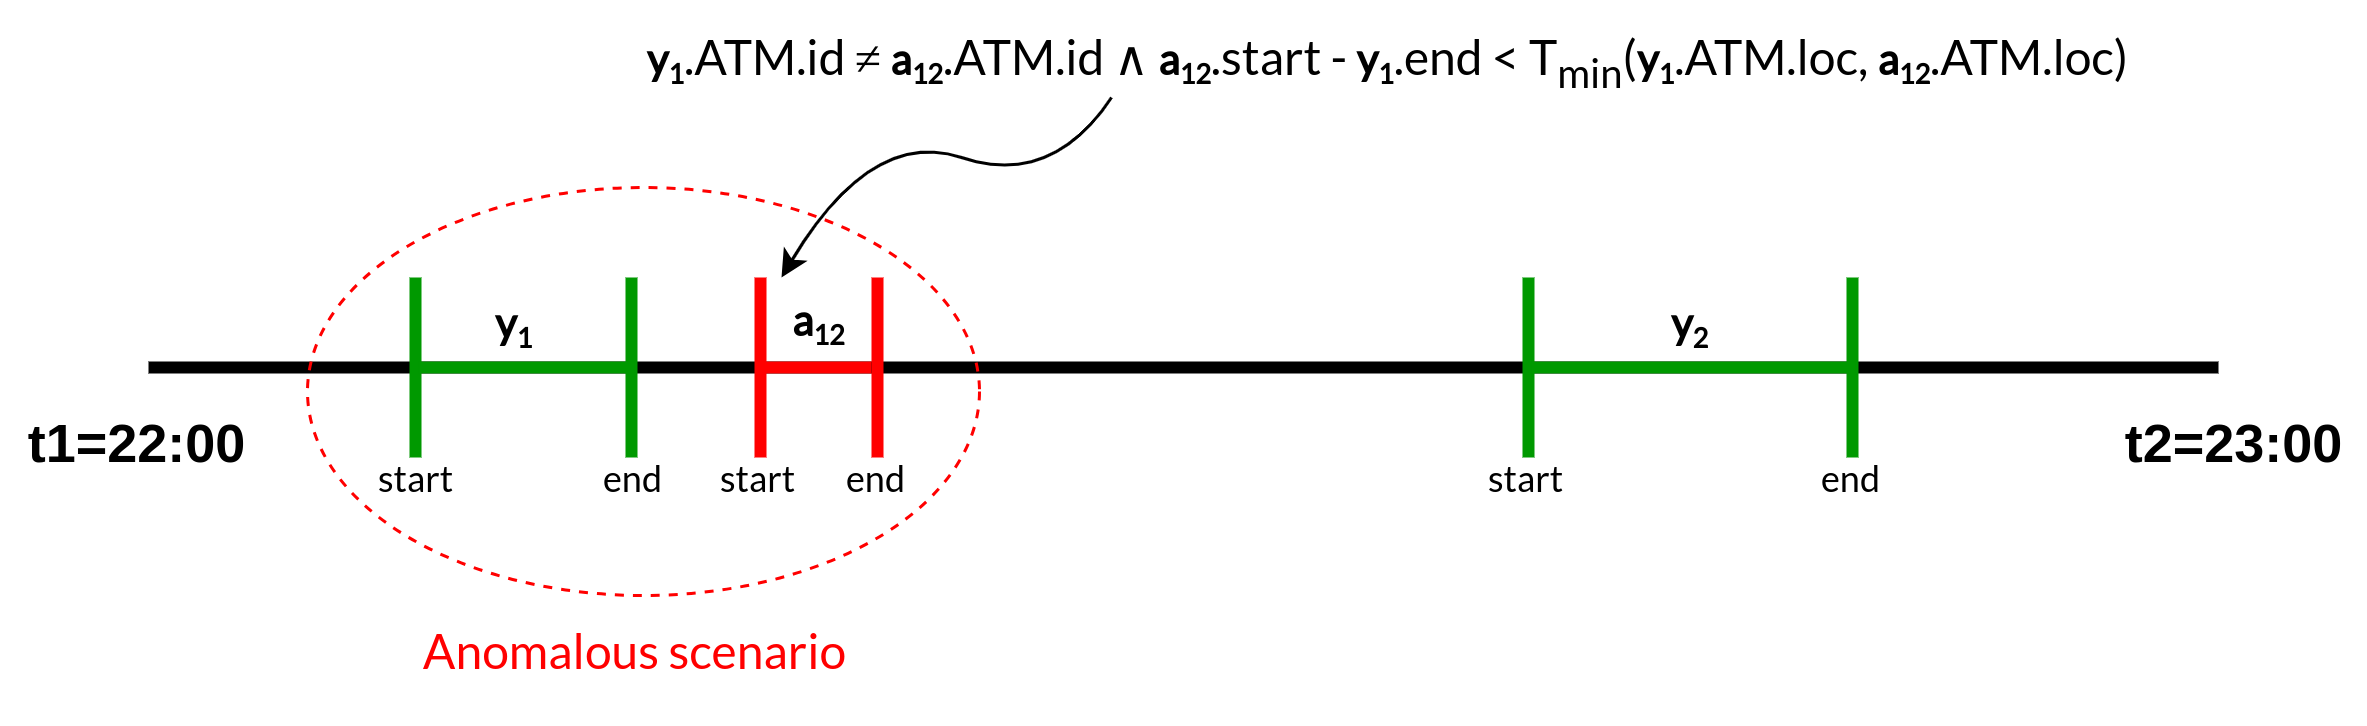
\includegraphics[width=\textwidth]{images/1-DataModel/tx-generation.png}
    \caption{Creation of an anomalous scenario of the fraud pattern type I}
    \label{img:anomalous-type-1}
\end{figure}

Some assumptions related with the generation of anomalous transactions were made: (i) Overlapping of transactions is not possible; (ii) There are no two consecutive anomalous transactions. Both assumptions were made for simplicity in order to avoid creating other fraud patterns apart from the one considered so far (fraud pattern I). Note that, these assumptions could be omitted otherwise.

\begin{itemize}
  \item \textbf{Overlapping of transactions is not possible}.
  Apart from guaranteeing that this injection causes at least one anomalous scenario, we also respect the additional constraint of ensuring that the anomalous transaction injected does not cause overlapping with any of the transactions, in particular neither with the previous nor the next one. Therefore considering that $a_{12}$ is the anomalous injected transaction in between the regular consecutive transactions $y_1$ and $y_2$, when generating $a_{12}$ we guarantee that:
  $$
  \begin{cases}
    a_{12}.\texttt{start} > y_{1}.\texttt{end} \\
    a_{12}.\texttt{end} < y_{2}.\texttt{start}
  \end{cases}
  $$
  \item \textbf{There are no two consecutive anomalous transactions}. For simplicity, in the generation of anomalous transactions we do not allow the injection of two or more consecutive anomalous transactions. That is, an anomalous transaction can only be injected between two regular consecutive transactions. See Figure \ref{img:anomalous-type-1-insertion-points}.
  \begin{figure}[H]
    \centering
    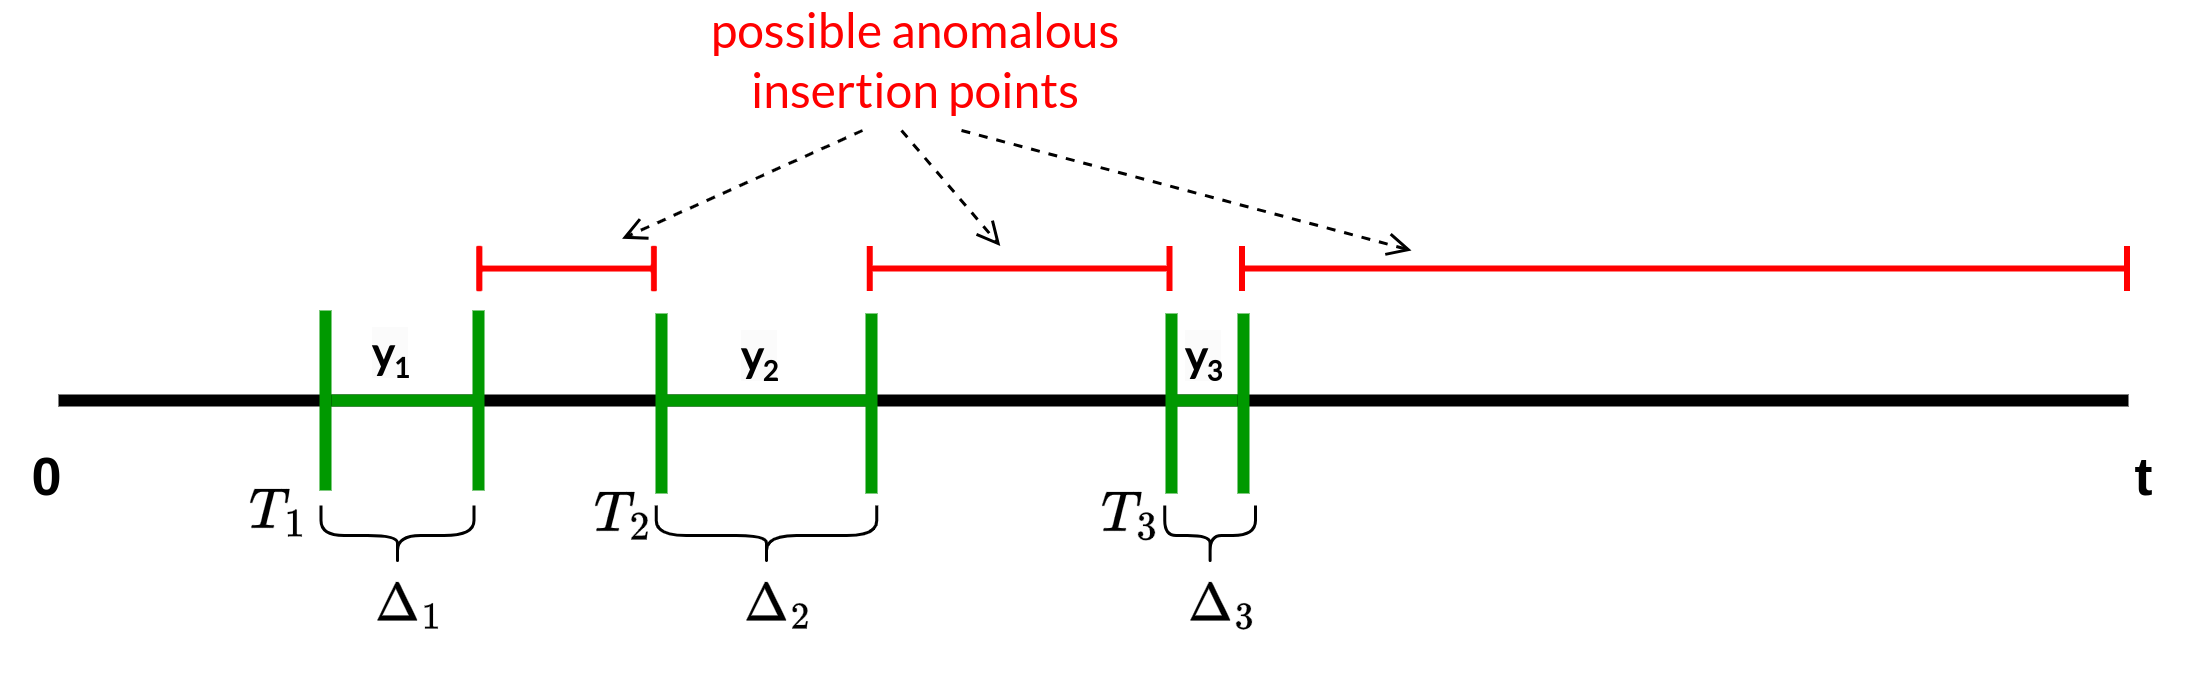
\includegraphics[width=\textwidth]{images/1-DataModel/tx-generation-anomalous-1.png}
    \caption{Considered possible injection points of anomalous transactions of fraud type I}
    \label{img:anomalous-type-1-insertion-points}
  \end{figure}  
\end{itemize}

$\texttt{ANOMALOUS\_RATIO\_1} \in [0,1]$ defines the ratio of anomalous transactions of the fraud pattern I over the total number of regular transactions \texttt{num\_tx} for each of the cards. So that $\texttt{ANOMALOUS\_RATIO\_1} * \texttt{num\_tx}$ is the number of injected anomalous transactions for each of the cards.\\

In Algorithm \ref{alg:anomalous-tx-generator-1} we describe at a high level the process of the generation of anomalous transactions for the fraud pattern I. This algorithm is run just after the generation of the regular transaction set, for each of the cards. 

\begin{algorithm}[H]
  \small
    \textbf{Precondition:} This algorithm is run just after the creation of the regular transaction set for each of the cards. $\texttt{ATM\_subset}$ and its complement $\overline{\texttt{ATM\_subset}}$ are provided as parameters from the regular transaction generator, for each of the cards.\\[5pt]
  $\textbf{introduceAnomalous}(\texttt{ATM\_subset}, \overline{\texttt{ATM\_subset}})$
  \begin{algorithmic}[1]
  \STATE $\texttt{num\_anomalous} \gets \texttt{num\_tx} * \texttt{ANOMALOUS\_RATIO\_1}$
  \STATE $i \gets 0$
  \WHILE{$i < \texttt{num\_anomalous}$}
      \STATE $\texttt{ATM}_{i} \sim \overline{\texttt{ATM\_subset}}$
      \STATE $prev_i, next_i \gets \text{randomUniquePosition(\texttt{num\_tx})}$
      \STATE $t_i \gets \text{getTime}(prev_i, next_i)$
      \STATE $\texttt{start}_{i} \gets t_i.start$
      \STATE $\texttt{end}_{i} \gets t_i.end$
      \STATE $\texttt{type}_{i} \gets \texttt{getRandomType()}$
      \STATE $\texttt{amount}_{i} \gets \texttt{getAmount()}$
      \STATE $\texttt{id}_{i} \gets \texttt{id}; \ \texttt{id} \gets \texttt{id} + 1$
      \STATE $\texttt{createTransaction}(\texttt{id}_{i}, \texttt{ATM}_i, \texttt{start}_{i},\texttt{end}_{i}, \texttt{type}_{i}, \texttt{amount}_i)$
      \STATE $i \gets i + 1$
  \ENDWHILE
  \end{algorithmic}
  \caption{Injection of Anomalous Transactions of Fraud Pattern I}
  \label{alg:anomalous-tx-generator-1}
\end{algorithm}


\begin{enumerate}
  \item \textbf{Assignment of ATMs not belonging to the \texttt{ATM\_subset}}: The anomalous transactions are linked to ATMs that are part of the complementary of the \texttt{ATM\_subset}, the $\overline{\texttt{ATM\_subset}}$.
  \item \textbf{Each anomalous transaction has a unique insertion position}: As described previously, we do not allow the case of two or more consecutive anomalous transactions injection. Each anomalous transaction occupies a unique position among all the possible injection positions defined by the set of regular transactions generated for the card. As it can be seen on Figure \ref{img:anomalous-type-1-insertion-points}, considering that we have three regular transactions, we will consider three unique possible insertion points for the anomalous transactions. The procedure of assigning a unique insertion position for each anomalous transaction to be generated is achieved with the function \text{randomUniquePosition(\texttt{num\_tx})}, that given the number of regular transactions of the card \texttt{num\_tx} returns the previous and the next regular transaction to the assigned unique position.
  \item \textbf{Assign transaction times respecting the needed time constraints}: In particular there are two time constraints to be satisfied:
  \begin{itemize}
    \item Produce fraud pattern I with $prev\_i$.
    \item No overlapping with $prev\_i$ nor with $next\_i$.
  \end{itemize}
  This is summarized in the pseudocode as the procedure getTime($prev\_i$, $next\_i$), which returns $t_i$, as the tuple of (\texttt{start}, \texttt{end}) times satisfying this two time constraints. To do it, we use the \texttt{ANOMALOUS\_SPEED} (in km/h) as the assumed maximum speed at which the distance between the two ATMs of the regular and the anomalous transactions can be traveled. The time distance between the regular and the anomalous injected transaction is calculated based on this assumed maximum speed. So that a fraud pattern I is intended to be produced if the distance between the two ATMs is covered at a faster speed than the \texttt{ANOMALOUS\_SPEED}, considered unfeasible. Finally \texttt{end} time is set as $\texttt{end} = \texttt{start} + \texttt{ANOMALOUS\_TX\_DURATION}$.
  \item \textbf{Random transaction type}: Since the specific transaction \emph{type} is not relevant for the production of the fraud pattern I, we assign it randomly (withdrawal, deposit, inquiry or transfer).
  \item \textbf{Arbitrary amount}: Similarly, this is not a relevant property for the fraud pattern I, and therefore we just assign it an arbitrary amount such as $prev_i.\texttt{transaction\_amount} * 2$.
\end{enumerate}

\paragraph{Transaction Stream Generator: \texttt{txGenerator.py}\\\\}

We implemented the aforementioned generator of the synthetic transaction streams as a Python program
\texttt{txGenerator.py}. On it we need to specify the value of the parameters needed to customize the generation of the stream of transactions. 
The customizable parameters and their description is provided in Table \ref{table:stream-generator-parameters}. To use it:

\begin{enumerate}
    \item Ensure to have a \texttt{csv} named directory with the \emph{csv} stable bank dataset files on which we want to simulate a transaction stream (use the bank data generator to produce it).
    \item Run \texttt{\$> python3 txGenerator.py <outputFileName>} introducing \emph{outputFileName} as an argument to name the transaction stream dataset files to be generated.
\end{enumerate}

The program generates a \texttt{tx} directory with the \emph{csv} files representing the transaction stream dataset:

\begin{itemize}
    \item \texttt{<outputFileName>-all.csv}: joint regular and anomalous dataset.
    \item \texttt{<outputFileName>-regular.csv}: regular transaction dataset.
    \item \texttt{<outputFileName>-anomalous.csv}: anomalous transaction dataset.
\end{itemize}

Finally, a simplified version of this synthetic stream generator was developed in the Python program \texttt{txGenerator-simplified.py}. On it, the \texttt{ATM\_subset} is built from a random selection of ATMs of the bank network, and not based on the distance to the residence location of the cardholder. This results in a faster generator, since it reduces the time complexity of the generation.

\begin{table}[H]
\hspace*{-1cm}
\centering
\renewcommand{\arraystretch}{1.2} % Increase row spacing
\begin{tabular}{|l|p{10cm}|} % Adjust second column width
\hline
\multicolumn{1}{|c|}{\textbf{Parameter}} & \multicolumn{1}{c|}{\textbf{Description}} \\ \hline
\texttt{START\_DATE} & Start date (in date format: \texttt{"YYYY-MM-DD"}) \\ \hline
\texttt{NUM\_DAYS} & Number of days duration of the transaction stream generated \\ \hline
\texttt{MAX\_DISTANCE\_SUBSET\_THRESHOLD} & Maximum allowed distance (in km) of the ATMs in the ATM subset to the client location residence \\ \hline
\texttt{MAX\_SIZE\_ATM\_SUBSET\_RATIO} & Ratio $\in [0,1]$ to limit the maximum size of the ATM subset from which regular transactions of a card are linked to. So that: 
$|\texttt{ATM\_subset}| = \texttt{MAX\_SIZE\_ATM\_SUBSET\_RATIO} * |\texttt{ATM}|$ \\ \hline
\texttt{MAX\_DURATION} & Maximum time (in seconds) duration of a transaction \\ \hline
\texttt{MEAN\_DURATION} & Mean duration (in seconds) duration of a transaction \\ \hline
\texttt{STD\_DURATION} & Standard deviation (in seconds) duration of a transaction \\ \hline
\texttt{REGULAR\_SPEED} & Assumed as the normal speed (in km/h) at which a client normally can travel the distance between two geographical points \\ \hline
\texttt{ANOMALOUS\_RATIO\_1} & Ratio $\in [0,1]$ of anomalous transactions of the fraud pattern I over the total number of regular transactions for each of the cards. \\ \hline
\texttt{ANOMALOUS\_SPEED} & Assumption on the maximum speed (in km/h) at which the distance between two geographical points can be traveled, for the generation of anomalous transactions \\ \hline
\texttt{ANOMALOUS\_TX\_DURATION} & Duration (in seconds) of an anomalous transaction \\ \hline
\end{tabular}
\caption{Description of the customizable parameters for the transaction stream generation}
\label{table:stream-generator-parameters}
\end{table}

% Apartado tamaños de banco y streams - que hemos generado / considerado para los experimentos
\subsection{Considered Datasets}\label{exps:considered-datasets}

Testing a bank system application like the \DPATM\ system implies deciding on different representative bank sizes and different stream configurations on which to perform the evaluation of the system. Regarding the stream of transactions the proportion of regular vs anomalous transactions also needs to be decided.\\

We propose two different bank databases: \smallG\  and \mediumG. \smallG\  simulates a small-sized bank database system, whereas \mediumG\ intends to simulate a large bank database; such as the \emph{Deutsche Bank Spain}\cite{DBSpain}. 
In table \ref{table:bank-dbs-details} we give their details on its number of Cards and ATM entities.

\begin{table}[H]
\centering
\begin{tabular}{|c|c|c|c|c|}
\hline
\textbf{Name} & \textbf{$|\text{Card}|$} & \textbf{$|\text{ATM}|$} & \textbf{$|\text{ATM}_{\text{Internal}}|$} & \textbf{$|\text{ATM}_{\text{External}}|$} \\ \hline
\smallG    & 2000      & 50     & 40        & 10        \\ \hline
\mediumG    & 500000      & 1000     & 900        & 100        \\ \hline
\end{tabular}
\caption{Considered bank databases characteristics}
\label{table:bank-dbs-details}
\end{table}

\subsubsection{Stream Configurations}\label{exps:bank-stream}
Regarding the design of the synthetic generated stream of transactions, 
we did a brief investigation of some related works, with respect to the stream sizes as well as the ratio on the anomalous fraud transactions they utilize.\\

On \cite{exps-atmfrauddetectionstreamdata} the authors propose an ATM fraud detection system based on ML models where they experiment with a transaction stream of a size close to $10^{6}$ consisting of a ratio of 0.88 regular operations to 0.12 fraudulent operations. In \cite{exps-costsensitivepayment} they propose a ML algorithm based on dynamic random forests and k-nearest neighbors, and they test it with a real bank transaction stream of $\sim5 \times 10^{4}$, representing the card activity of 415 different cards, with a fraudulent transaction ratio of 0.07. Finally, in \cite{exps-featureengineering} they evaluate the impact of their proposed feature extraction techniques for credit card fraud detection on different ML and data mining state-of-the-art models. For their experiments they used a real European transaction dataset containing $\sim120 \times 10^{6}$ transactions representing a 18 months time interval, in which only $\sim40000$, that is a $0.025\%$, are fraudulent. They also consider a smaller subset of $\sim 2 \times 10^{5}$ transactions with a fraud ratio of $1.5\%$.\\

Based on these references, for each considered bank database; \smallG\ and \mediumG, we constructed different streams with sizes and fraud ratio similar to the ones mentioned, using our generator of synthetic transactions, generated from different bank databases. When generating the streams, in order to obtain the desired stream sizes, we needed to consider that our transaction generator takes as base the behavior of the clients of the \emph{Wisabi Bank Database}, where each client typically produces less than 1 transaction operation per day, in particular $\mathsf{0.666}$ transactions per day per cardholder on average (see table \ref{table:wisabi-average-num-ops}). This means that for each of the bank sizes being tested, in order to achieve the desired stream size, we needed to decrease/increase the size of the time interval to be simulated.\\

Table \ref{table:stream-sizes} presents summary of the details on the different transactions streams generated for each of the bank databases. The customizable parameter values that we used for the generation of these streams are detailed in table \ref{table:stream-generator-parameters-specific}. All the generated streams were generated with those same common parameter values. The parameters that varied were: the \texttt{NUM\_DAYS} to regulate the length of the transaction stream generated; and the \texttt{ANOMALOUS\_RATIO\_1}, to vary the ratio of anomalous transactions generated.

\begin{table}[H]
    \small 
    \hspace*{-1cm}
    \centering
    \begin{tabular}{|l|c|c|c|c|c|c|}
    \hline
    \textbf{Name} & \textbf{Bank DB} & \textbf{$|\text{Days}|$} & \begin{tabular}[c]{@{}c@{}}\textbf{Anomalous}\\ \textbf{Ratio}\end{tabular} & \textbf{Stream Size} & \textbf{$|\text{Regular Tx}|$} & \textbf{$|\text{Anomalous Tx}|$} \\ \hline
    $\mathsf{GDB_A\text{-}30}$ & \smallG    & 30       & $0.02\ (2\%)$   & 39959       & 39508      & 451   \\ \hline
    $\mathsf{GDB_A\text{-}60}$ & \smallG     & 60       & $0.02\ (2\%)$   & 80744       & 79005      & 1739         \\ \hline
    $\mathsf{GDB_A\text{-}120}$ & \smallG     & 120      & $0.02\ (2\%)$   & 160750      & 157756     & 2994         \\ \hline
    $\mathsf{GDB_B\text{-}7}$ & \mediumG    & 7        & $0.03\ (3\%)$   & 2428286     & 2401806    & 26480        \\ \hline
    $\mathsf{GDB_B\text{-}15}$ & \mediumG    & 15       & $0.03\ (3\%)$   & 4856573     & 4805920    & 50653        \\ \hline
    \end{tabular}
    \caption{Summary of the different streams generated for each of the bank databases. For each stream, we indicate the time interval (in days) that it simulates, the anomalous ratio, its exact stream size (in the number of transactions), and from it, its number of regular and only anomalous transactions.}
    \label{table:stream-sizes}
\end{table}

As a remark, note that for the \mediumG\ we utilized the simplified version of the generator, whereas for the \smallG\ we utilized the original version.

\begin{table}[H]
\hspace*{-1cm}
\centering
\renewcommand{\arraystretch}{1.2} % Increase row spacing
\begin{tabular}{|l|l|} % Adjust second column width
\hline
\multicolumn{1}{|c|}{\textbf{Parameter}} & \multicolumn{1}{c|}{\textbf{Value}} \\ \hline
\texttt{START\_DATE} & 2018-04-01 \\ \hline
\texttt{MAX\_DISTANCE\_SUBSET\_THRESHOLD} & 70 (km)\\ \hline
\texttt{MAX\_SIZE\_ATM\_SUBSET\_RATIO} & 0.2\\ \hline
\texttt{MAX\_DURATION} & 600 (s)\\ \hline
\texttt{MEAN\_DURATION} & 300 (s) \\ \hline
\texttt{STD\_DURATION} & 120 (s) \\ \hline
\texttt{REGULAR\_SPEED} & 50 (km/h) \\ \hline
\texttt{ANOMALOUS\_SPEED} & 500 (km/h) \\ \hline
\texttt{ANOMALOUS\_TX\_DURATION} & 5 (s) \\ \hline
\end{tabular}
\caption{Description of the values used for the customizable parameters of the transaction stream generator for the generated streams}
\label{table:stream-generator-parameters-specific}
\end{table}

\subsection{Stream Ingestion}\label{exps-input-reading}

As it was already advanced in the description of the implementation of the \source\ \Sr\ stage in \ref{sec:CQE-DPATM}, the way the stream of interactions is input into the \DPATM\ system is of paramount importance when evaluating the performance of a real-time system like ours.\\

In a real-case scenario, the interaction/transaction events coming from the network of ATMs of the bank would be typically received in a stream manner by a message queue of the \DPATM\ system. However, to test our proof of concept \DPATM\ system, we decided to simplify this process and do a file input read of the \texttt{csv} files containing our generated simulated synthetic transaction streams. The interactions are read from these files, parsed into \texttt{Edge} data types and provided to the pipeline in different ways depending on the kind of simulation we perform. \\

For all the kinds of experiments we perform we want the reading of the input file to be the fastest possible, so to minimize the potential bottleneck derived from the I/O operation of reading a file. With this purpose, we utilized a buffered reader of the \texttt{bufio} package, which reads chunks of data into memory, providing buffered access to the file. This buffered reader was provided to a \texttt{csv} reader of the \texttt{encoding/csv} package to read the buffered stream as \texttt{csv} records.


    \begin{center}
    \lstset{style=golangStyle}
    \begin{lstlisting}[caption={\texttt{csv-bufio} reader}]
        reader := csv.NewReader(bufio.NewReader(file))
    \end{lstlisting}
    \end{center}
    
% Lectura por chunks
% chunk size = 100
% read with the help of a worker to keep reading in the background, to accelerate the reading -> explain the reason of why this
Another optimization that was done in order to be able to minimize this bottleneck on the reading of the interactions from the \texttt{csv} file, was reading by chunks the \texttt{csv} records/rows. In particular, this was done by having a \textit{worker} subprocess, implemented as an anonymous \texttt{goroutine} inside \Sr, whose task was to continuously read records from the file using the \texttt{csv-bufio} reader accumulating them in a chunk of rows that were provided through a channel to \Sr\ whenever they reached the defined \emph{chunkSize}. These records were read directly as \texttt{string} data types. On its side, whenever \Sr\ received a chunk of rows, it takes each of the rows on it, parses it to the \texttt{Edge} data type and sends it through the pipeline to the next stage. The \emph{chunkSize} was selected to be of $10^2$ rows.\\

The justification of the usage of this buffered and chunked file reading using the \texttt{encoding/csv} package with a \emph{chunkSize} of $10^2$ rows is provided with the upcoming results. On them the \texttt{encoding/csv} package performance is compared to other variants using the \texttt{apache/arrow} package with different combinations of \emph{chunkSize}. We also analyze the benefits of introducing the \textit{worker} subprocess to perform the chunked reading.\\

Some references that we utilized include: \cite{exps-input-read-go_apache_arrow, exps-input-read-apache_arrow_go_match, exps-input-read-apache_arrow_medium, exps-input-read-golang_arrow_voltrondata} are different blogs and tutorials where \texttt{Apache Arrow} is explained and where its usage with \texttt{Go} is also exemplified.
\cite{exps-chunk-by-chunk-reading} is an informal post where they experimentally showed some of the benefits of file reading in chunks.\\

% 1. comparison of csv/encoding with the other variants
First the performance of the \texttt{encoding/csv} package is compared to the \texttt{apache/arrow} package. \texttt{encoding/csv} \cite{go-encoding-csv} is the package provided by the \texttt{Go} standard library to decode and encode data using \texttt{csv} values format.
% describo apache/arrow - era con bufio? comprobar
\texttt{apache/arrow} \cite{apache-arrow-go} is a \texttt{Go} package from the \texttt{Arrow} platform \cite{apache-arrow-platform} that allows reading \texttt{csv} files in chunks of $n$ rows, called \emph{records}. An inconvenient is that \texttt{Apache Arrow} is optimized storing the data in a columnar way (by columns). So that we can not access the original $n$ rows easily, but instead the columns of these rows. And therefore, from them we will need to reconstruct the rows by taking the corresponding elements from each of the columns, given the index of the corresponding row.\\

All the compared approaches do the reading by chunks in a worker subroutine. The chunks are then provided to the main process through an internal communication channel. This intends to simulate a real implementation of the \source\ \Sr\ stage.

\begin{itemize}
  \item \texttt{apache/arrow-1}: Reading done with \texttt{apache/arrow} package. The worker performs the reading of each field of the \texttt{csv} with its corresponding data type. After reading a chunk, it is then transposed back to obtain the \texttt{Edge} type rows (as the library optimizes saving the \texttt{csv} by columns when read), and the chunk of \texttt{Edge} rows given to the main process. 
  \item \texttt{apache/arrow-2}: Reading done with \texttt{apache/arrow} package. The worker reads each field as \texttt{string} data type. After reading a chunk, it is transposed bank to row form and sent to the main process. The conversion to the corresponding \texttt{Edge} types is performed in the main process.
  \item \texttt{csv/encoding}: Reading done using the \texttt{encoding/csv} package. Row by row reading by the worker. When a chunk of rows is formed it passes it to the main process and the rows are then converted to \texttt{Edge}'s.
\end{itemize}

To perform these experiments we generated \texttt{csv} stream files of toy interactions of different sizes: $10^4$, $10^5$ and $10^6$ number of interactions (rows). For each of the sizes we compared the time it took to read the full file to each of the variants, also testing with different chunk sizes in terms of the number of rows: ranging from $10^0, 10^1, 10^2...$ up to the total number of rows of the file (maximum possible chunk size, i.e. all at once). Each of the experiments performed were run a total of 20 times to obtain stable measurements. The results can be seen in Figure \ref{img:exps-read-input-variants}. In all of the cases, the fastest approach is the variant using \texttt{encoding/csv} with chunk size \emph{chunkSize} of $10^2$ rows.\\

\begin{figure}[H]
  \centering
  \begin{minipage}{0.48\textwidth}
    \centering
    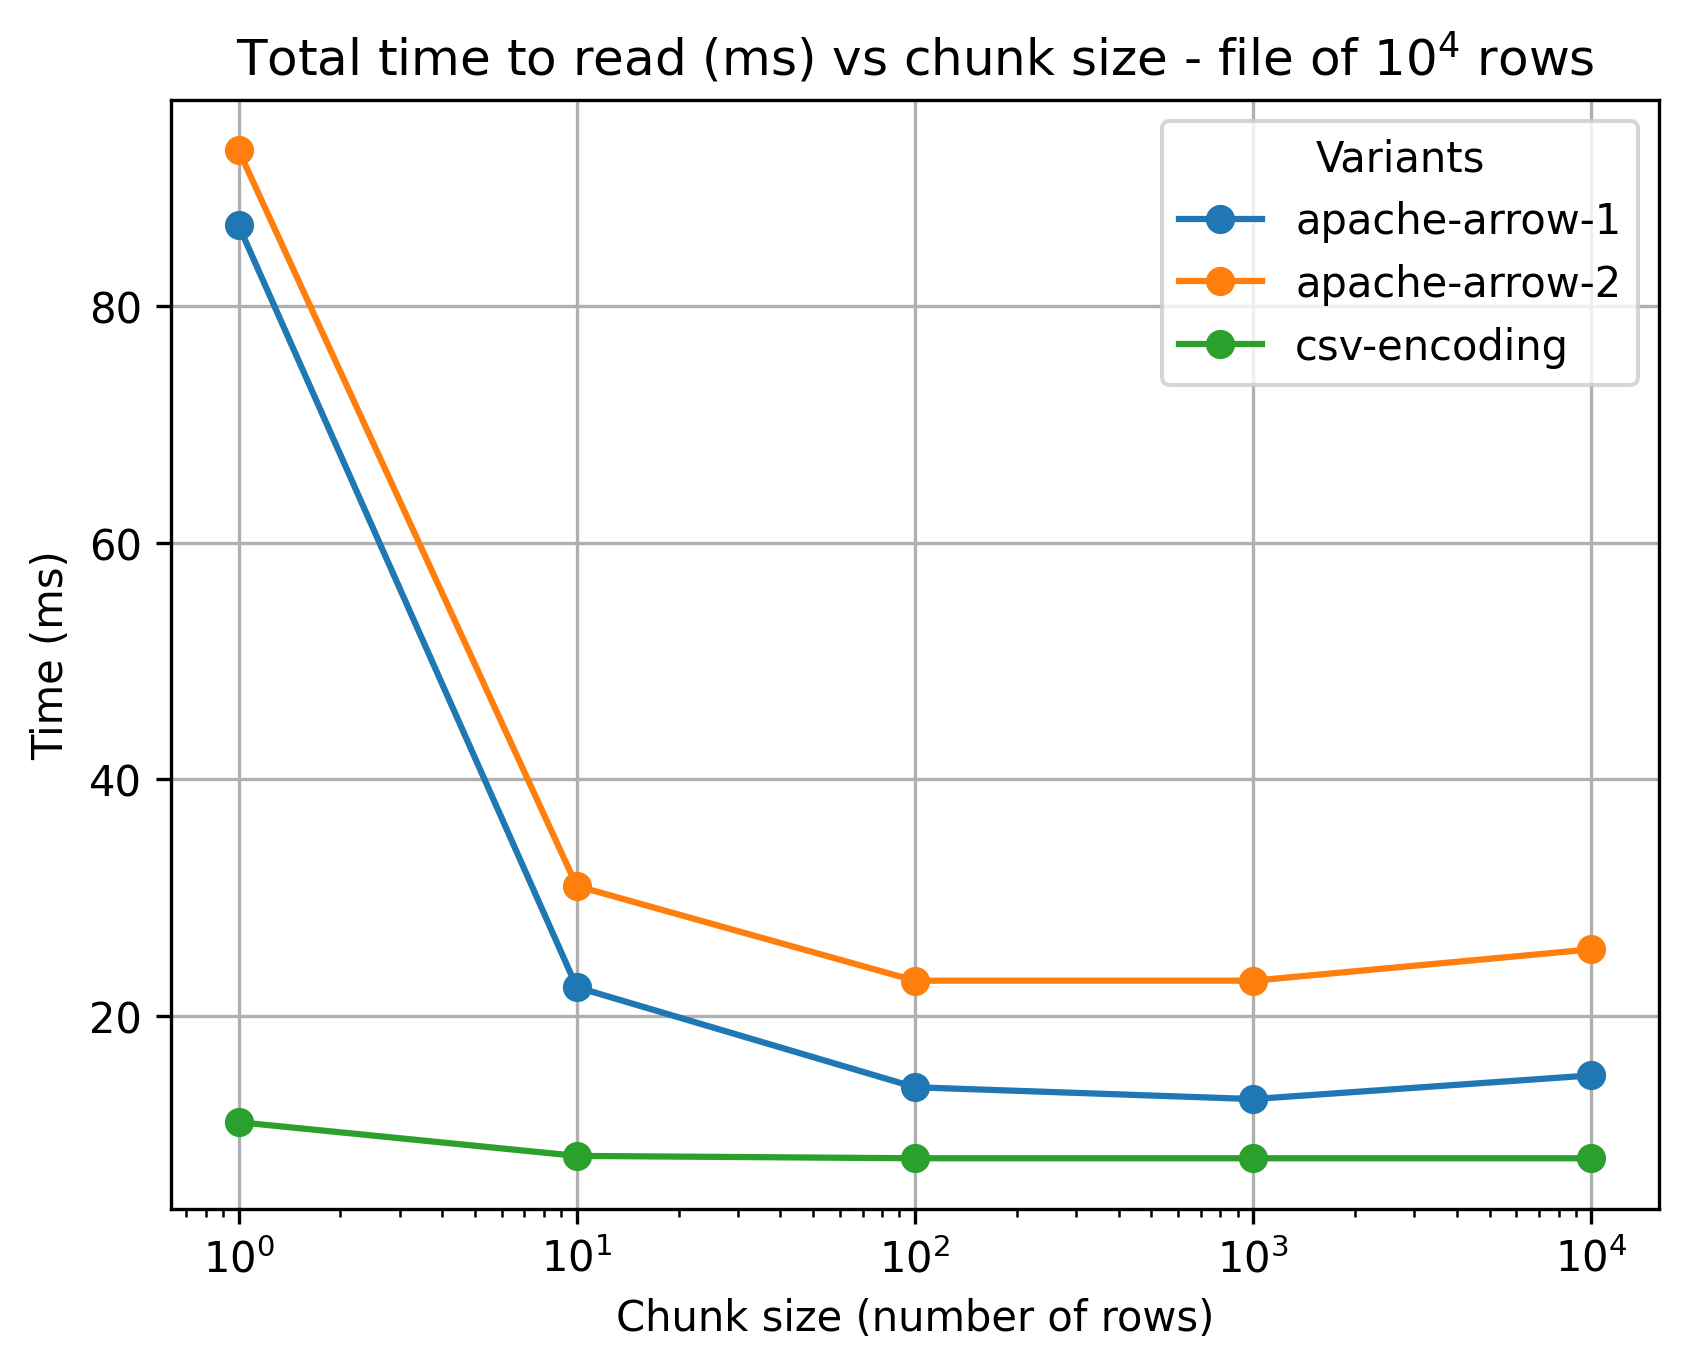
\includegraphics[scale = 0.5]{images/4-Experiments/read-input-10-4.png}
    \caption*{Test for \texttt{csv} file of size $10^4$ rows}
  \end{minipage}
  \hfill
  \begin{minipage}{0.48\textwidth}
    \centering
    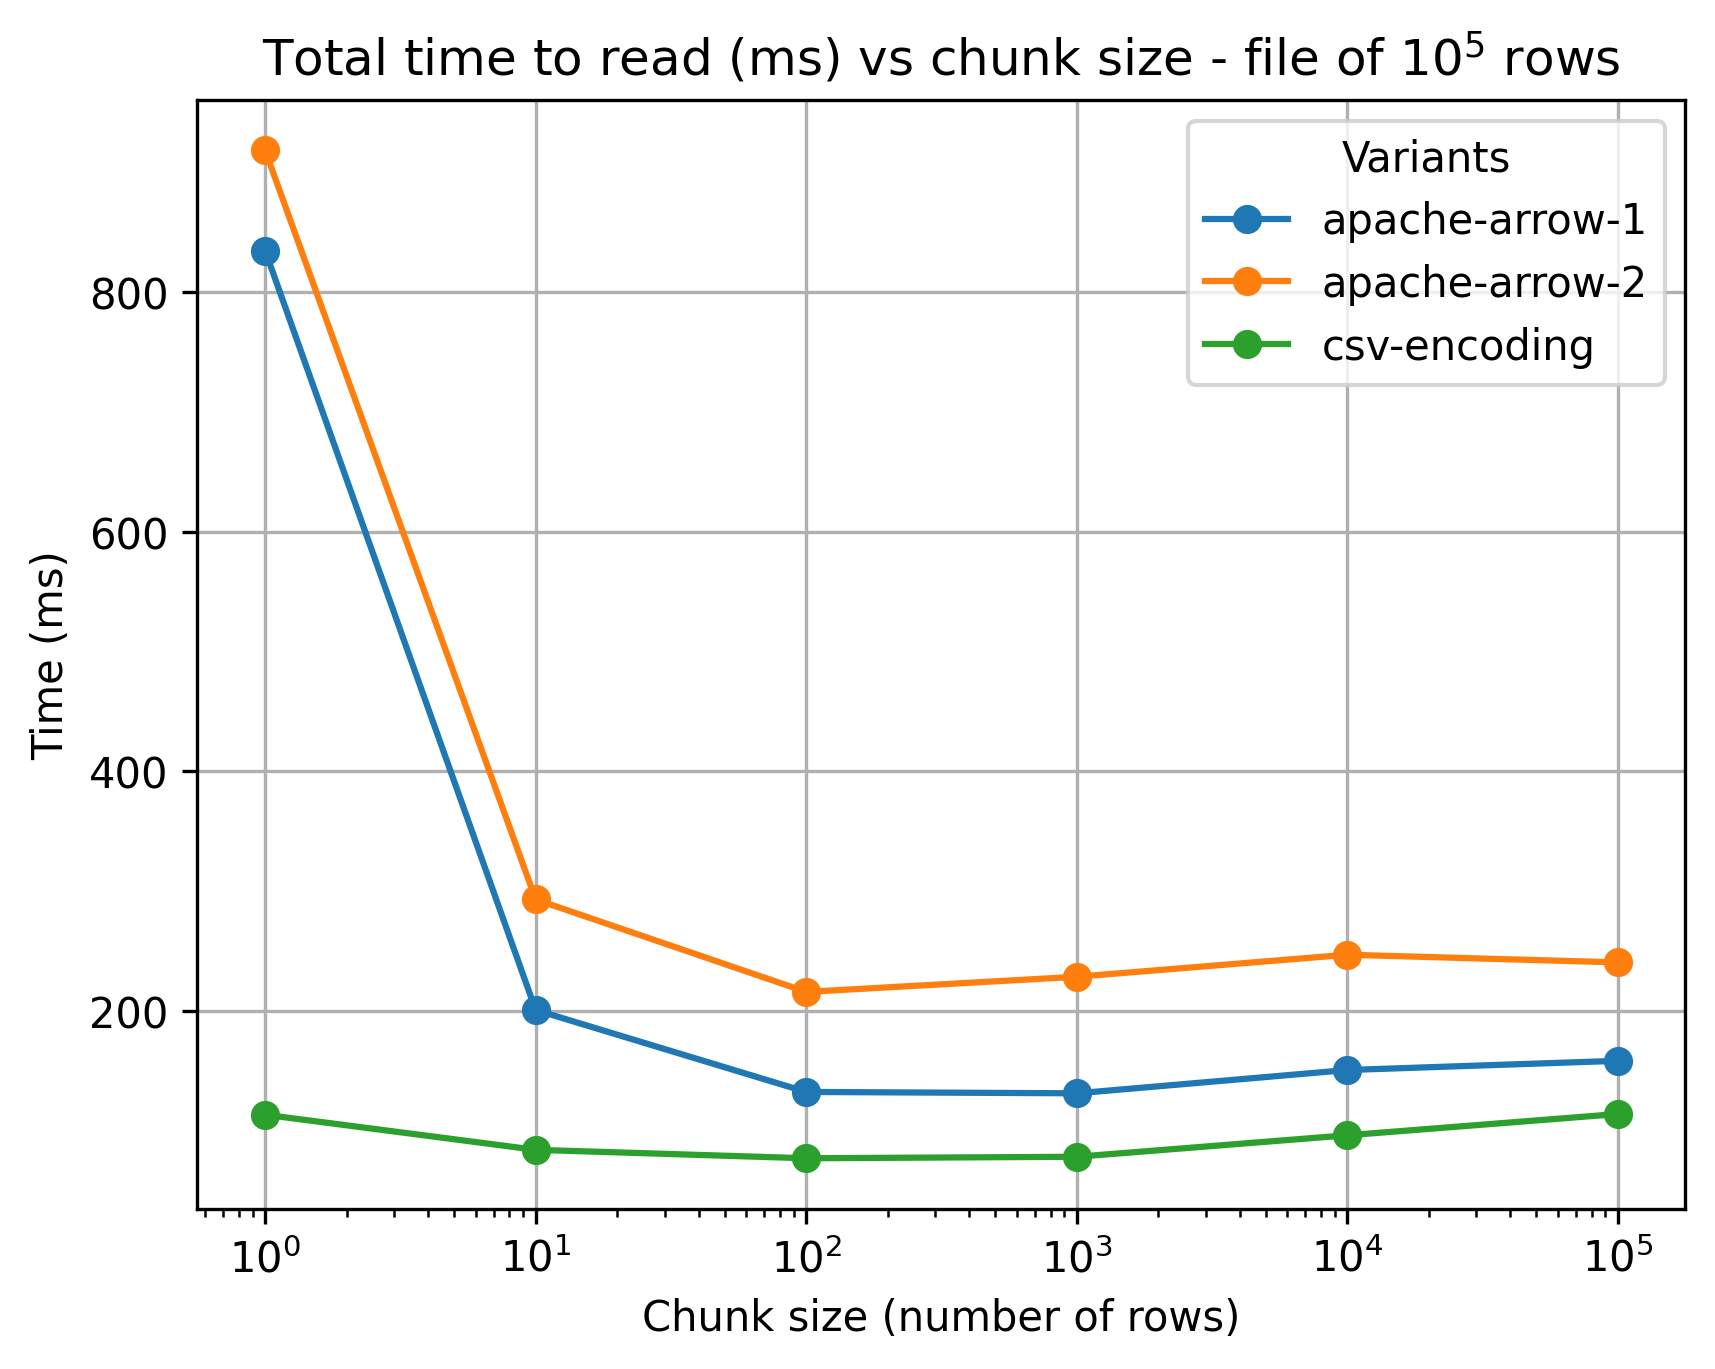
\includegraphics[scale = 0.5]{images/4-Experiments/read-input-10-5.png}
    \caption*{Test for \texttt{csv} file of size $10^5$ rows}
  \end{minipage}
  
  \vspace{0.5cm} % Add some vertical space between the rows

  \begin{minipage}{0.6\textwidth}
    \centering
    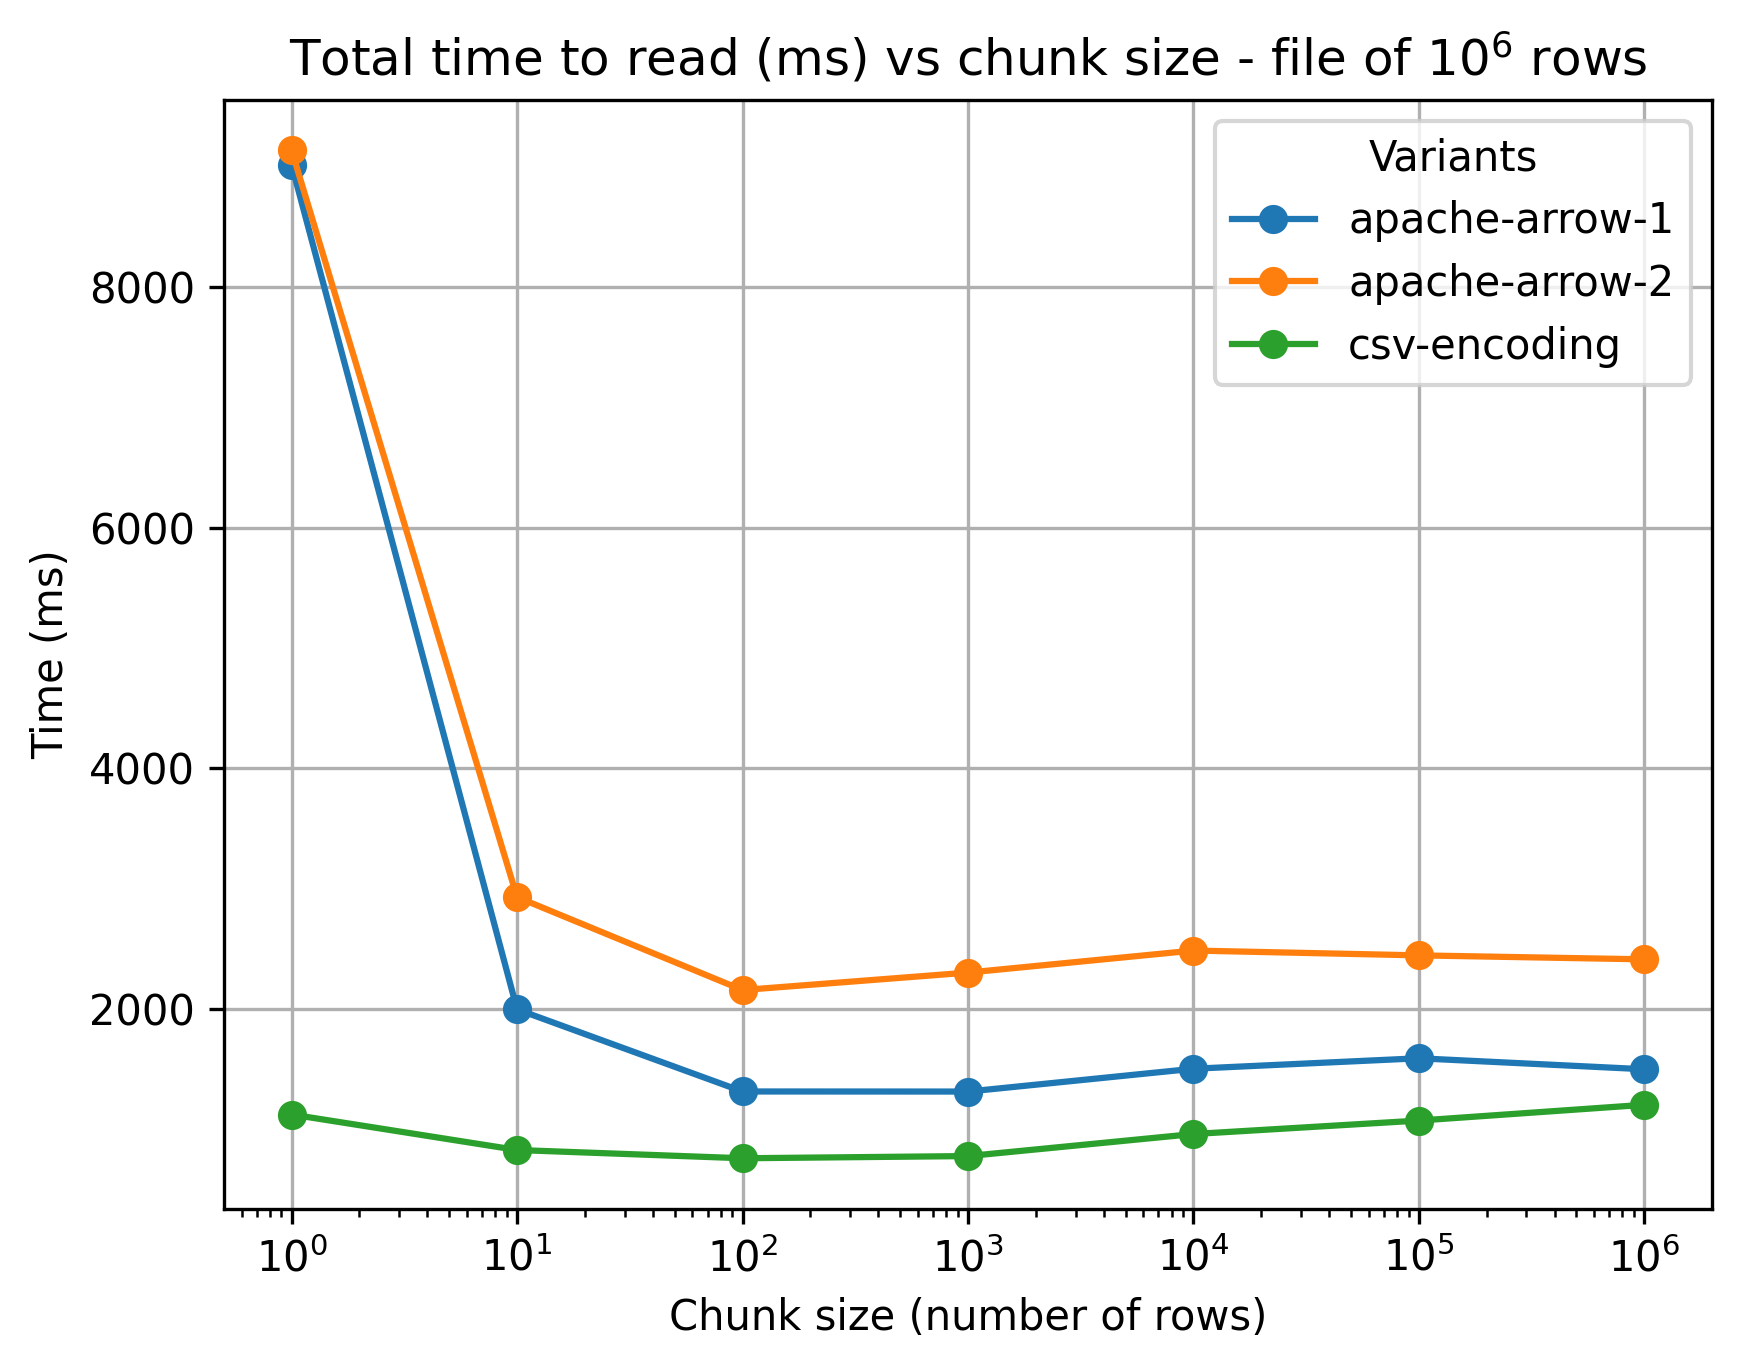
\includegraphics[scale = 0.5]{images/4-Experiments/read-input-10-6.png}
    \caption*{Test for \texttt{csv} file of size $10^6$ rows}
  \end{minipage}
  \caption{Comparison of the \texttt{apache/arrow-1}, \texttt{apache/arrow-2} and \texttt{encoding/csv} variants for reading different \texttt{csv} file sizes, using different chunk sizes.}
  \label{img:exps-read-input-variants}
\end{figure}

% 2. comparison of the benefits of no-worker vs worker with the csv/encoding
Once we decided to use the approach using the \texttt{encoding/csv} package, we performed an additional experiment in order to see if it was actually worthy to do the \emph{background} reading of the input with the worker subprocess \texttt{goroutine}. To see this we performed some experiments in which we compared the variant with worker and chunk size of $10^2$ with respect to the one without worker and without chunk reading. Again we compared the time it took to read \texttt{csv} interaction files of different sizes : from $10^4$ up to $10^6$ and $10^7$ rows/interactions. Each experiment was done 20 times to obtain stable measurements.\\

As it can be seen in Figure \ref{img:exps-csv-encoding-variants}, the differences are insignificant. Up to $10^6$ rows the variant with worker and chunk reading seems to be slightly better, although for the experiment with $10^7$ rows is the other way around.

\begin{figure}[H]
  \centering
  \begin{minipage}{0.49\textwidth}
    \centering
    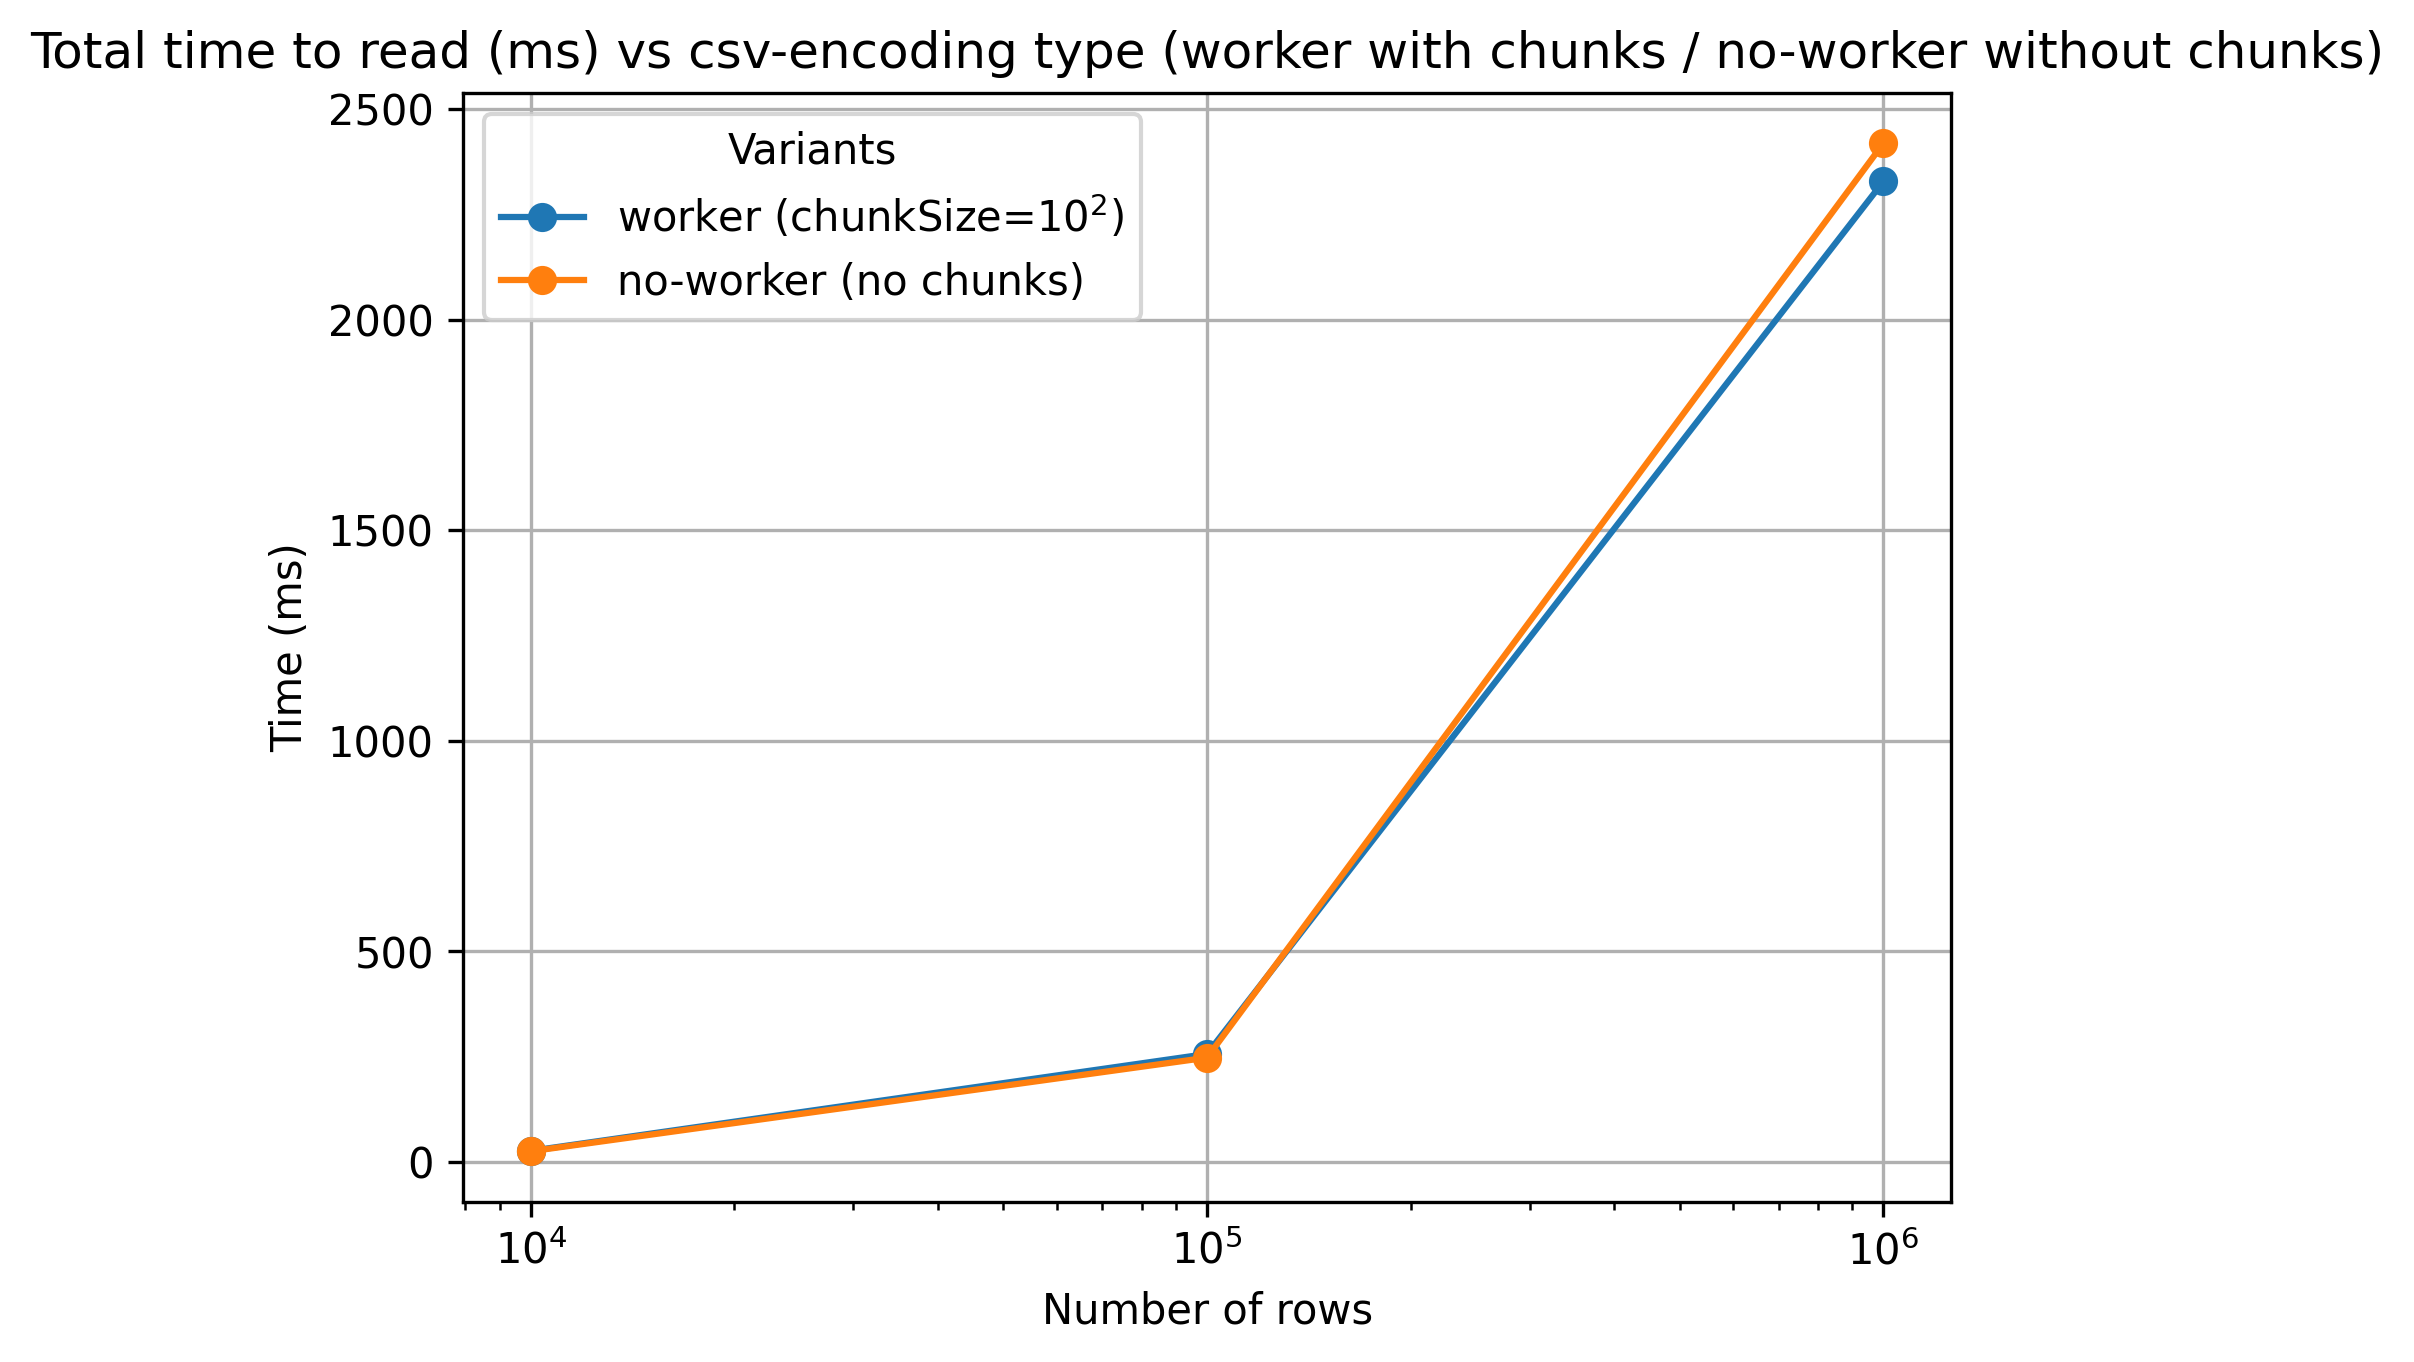
\includegraphics[scale = 0.46]{images/4-Experiments/read-input-csv-encoding.png}
    \caption*{Test for \texttt{csv} file of size up to $10^6$ rows}
  \end{minipage}
  \hfill
  \begin{minipage}{0.49\textwidth}
    \centering
    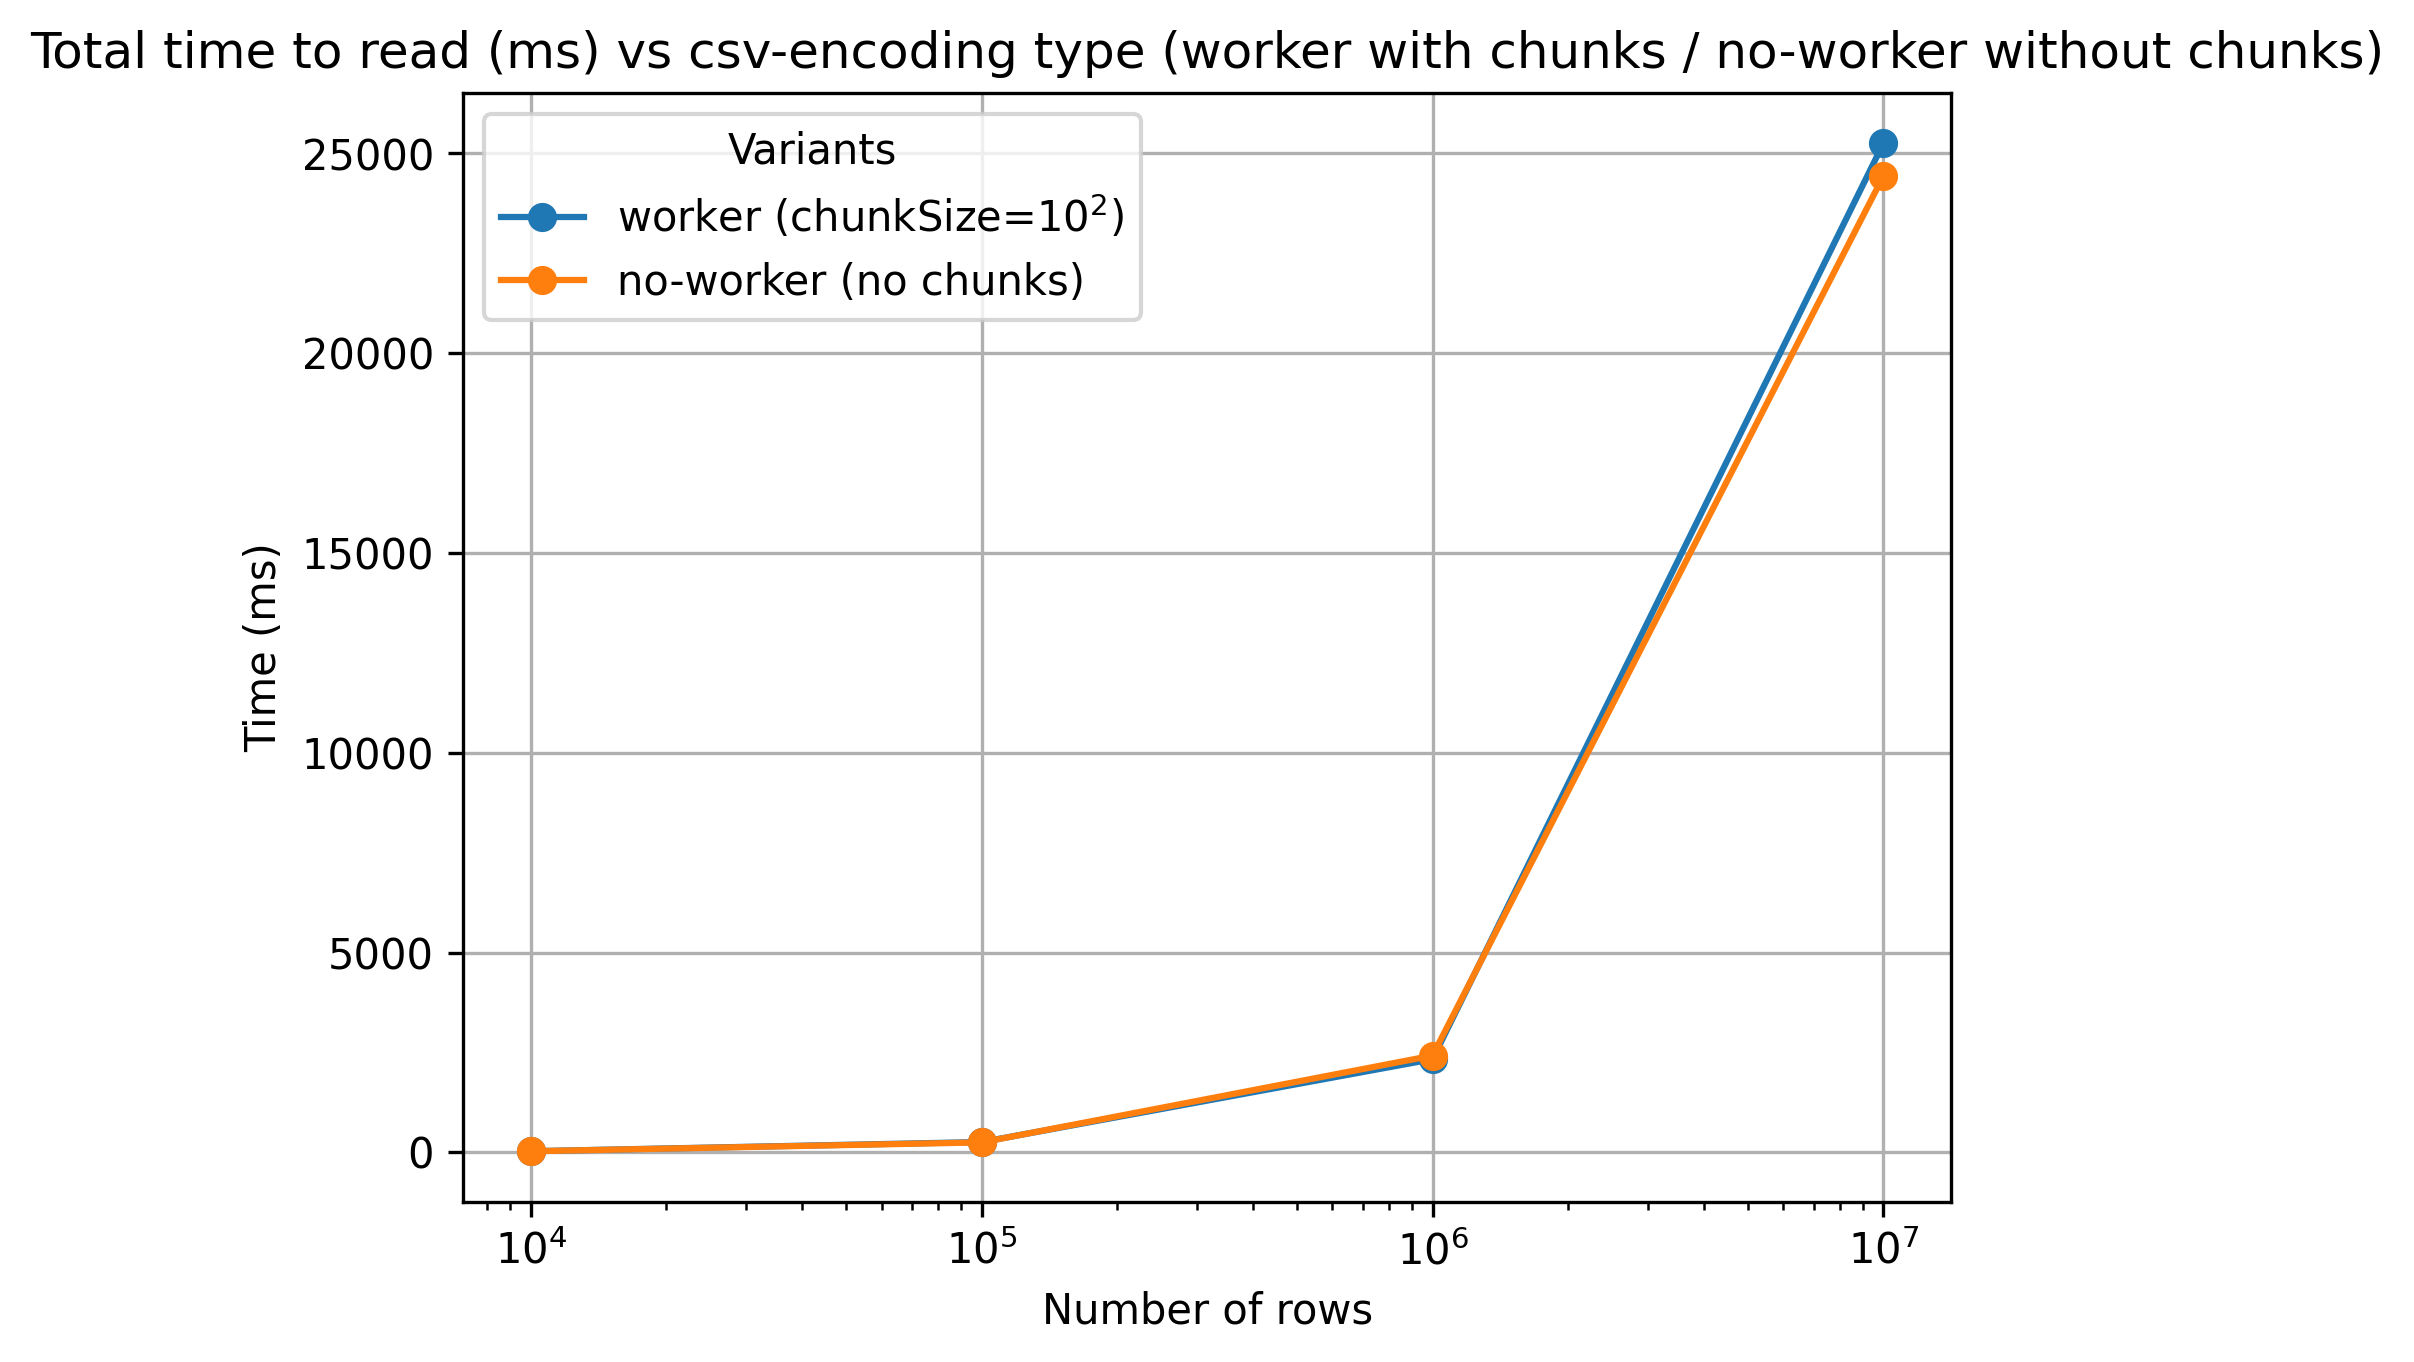
\includegraphics[scale = 0.46]{images/4-Experiments/read-input-csv-encoding-all.png}
    \caption*{Test for \texttt{csv} file of size up to $10^7$ rows}
  \end{minipage}
    \caption{Comparison of the worker and no worker variants using \texttt{encoding/csv} for reading different \texttt{csv} file sizes.}
    \label{img:exps-csv-encoding-variants}
\end{figure}

All these experiments were run with 1 core and 1024MB of RAM at the nodes of the RDLab-UPC cluster.
